\documentclass[newPxFont,numfooter,sectionpages]{beamer}
\usepackage[utf8]{inputenc}
\usepackage{hyperref}
\hypersetup{colorlinks=true, urlcolor=blue}
\usetheme{sthlm}
\usepackage{pgfplots}
\pgfplotsset{compat=1.14}
\usepackage{cancel}
\usepackage{animate}

%-=-=-=-=-=-=-=-=-=-=-=-=-=-=-=-=-=-=-=-=-=-=-=-=
%
%	PRESENTATION INFORMATION
%
%-=-=-=-=-=-=-=-=-=-=-=-=-=-=-=-=-=-=-=-=-=-=-=-=

\title{Bayesian estimation of time-trees:}
\subtitle{A journey through a strange land}
% \date{\today}
\author{Luiz Max Carvalho}
\institute{ Institute of Evolutionary Biology \\ Maxwell Institute seminar series 2017 }

\hypersetup{
pdfauthor = {LMCarvalho: lm.carvalho@ed.ac.uk},
pdfsubject = {MCMC},
pdfkeywords = {Bayesian statistics, phylogenetics, MCMC},
pdfmoddate= {D:\pdfdate},
pdfcreator = {}
}

\begin{document}

%-=-=-=-=-=-=-=-=-=-=-=-=-=-=-=-=-=-=-=-=-=-=-=-=
%
%	TITLE PAGE
%
%-=-=-=-=-=-=-=-=-=-=-=-=-=-=-=-=-=-=-=-=-=-=-=-=

\maketitle

%-=-=-=-=-=-=-=-=-=-=-=-=-=-=-=-=-=-=-=-=-=-=-=-=
%	FRAME: Acks
%-=-=-=-=-=-=-=-=-=-=-=-=-=-=-=-=-=-=-=-=-=-=-=-=
\begin{frame}{Acknowledgements}
\begin{columns}
\begin{column}{0.3\textwidth}
    \begin{figure}
     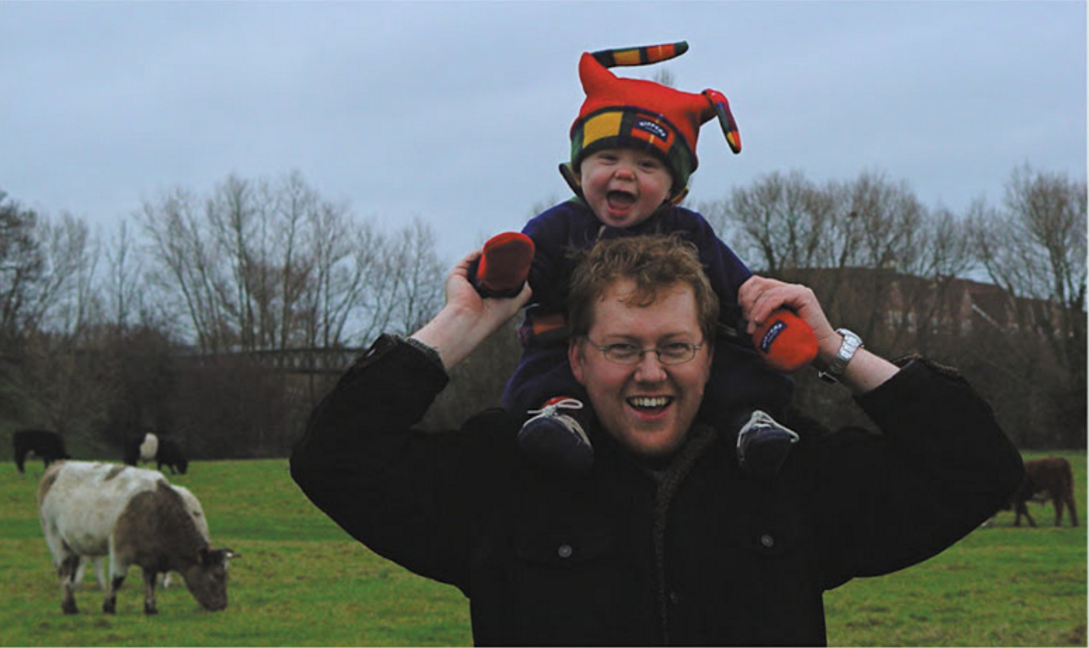
\includegraphics[width=\textwidth]{figures/rambaut.png} \\
     Andrew Rambaut \\
     UoE
     \end{figure}
\end{column}
\begin{column}{0.3\textwidth}  %%<--- here
    \begin{figure}
     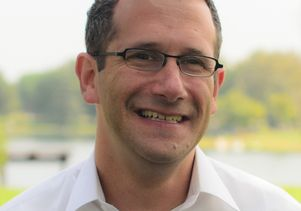
\includegraphics[width=\textwidth]{figures/suchard.png} \\
     Marc Suchard \\
     UCLA
     \end{figure}
\end{column}
\begin{column}{0.3\textwidth}  %%<--- here
    \begin{figure}
     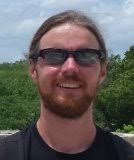
\includegraphics[width=\textwidth]{figures/baele.png} \\
     Guy Baele \\
     KU Leuven
     \end{figure}
\end{column}
\end{columns}
\end{frame}

%-=-=-=-=-=-=-=-=-=-=-=-=-=-=-=-=-=-=-=-=-=-=-=-=
%	FRAME: Outline
%-=-=-=-=-=-=-=-=-=-=-=-=-=-=-=-=-=-=-=-=-=-=-=-=
\begin{frame}{Plan for today}
\begin{alertblock}{Problem}
What are trees and why are interested in them?
\end{alertblock}%\pause
\begin{exampleblock}{Parameter space}
What does the space we are trying to sample look like?
\end{exampleblock}%\pause
\begin{block}{MCMC in tree space}
 A journey through a strange land
\end{block}%\pause
\begingroup
\setbeamercolor{block title}{fg=white, bg=\cnPurple}
\setbeamercolor{block body}{bg=\cnLightPurple}
\begin{block}{Preliminary results and perspectives}
Performance analyses and open problems.
\end{block}
\endgroup
\end{frame}

%-=-=-=-=-=-=-=-=-=-=-=-=-=-=-=-=-=-=-=-=-=-=-=-=
%	FRAME: Motivation
%-=-=-=-=-=-=-=-=-=-=-=-=-=-=-=-=-=-=-=-=-=-=-=-=
\begingroup
\begin{frame}{Motivation}
\begin{block}{Phylodynamics of fast-evolving viruses}
 Inferring spatial and temporal dynamics from genomic data:
 \begin{center}
  \Large \textbf{Phylogenies}$^\ast$! \\
  \tiny $^\ast$ plus complicated models
 \end{center}
\end{block}
\begin{figure}
	\centerline{
	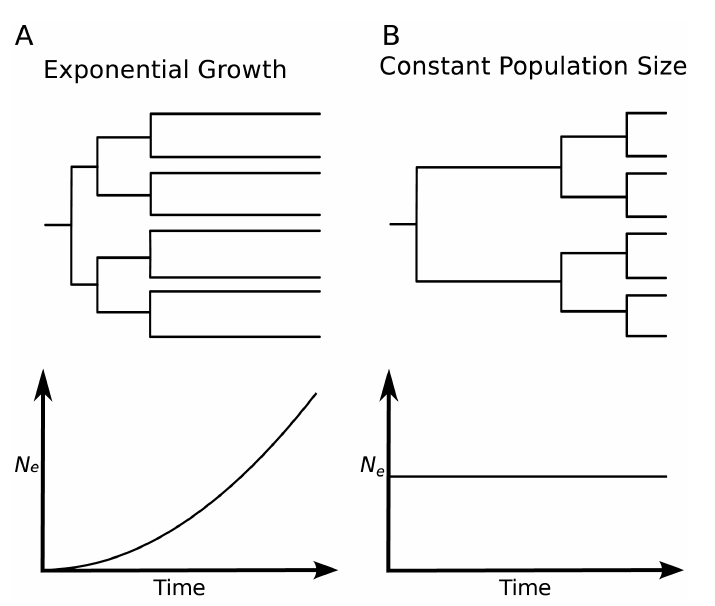
\includegraphics[width=0.5\textwidth,height=5cm]{figures/pop_growth.jpg}  
	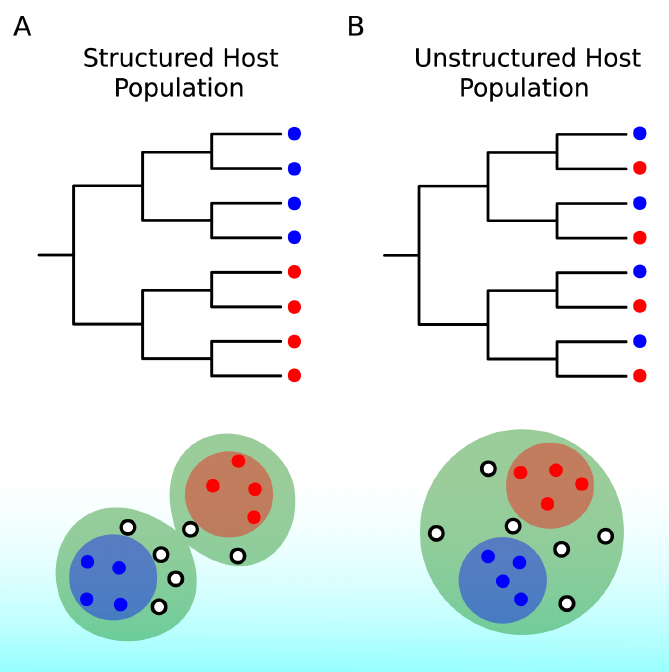
\includegraphics[width=0.5\textwidth,height=5cm]{figures/pop_structure.jpg}
	}
\end{figure}
\end{frame}
\endgroup

%-=-=-=-=-=-=-=-=-=-=-=-=-=-=-=-=-=-=-=-=-=-=-=-=
%	FRAME: coalescent
%-=-=-=-=-=-=-=-=-=-=-=-=-=-=-=-=-=-=-=-=-=-=-=-=
\begin{frame}{Trees and the coalescent}
\begin{figure}
	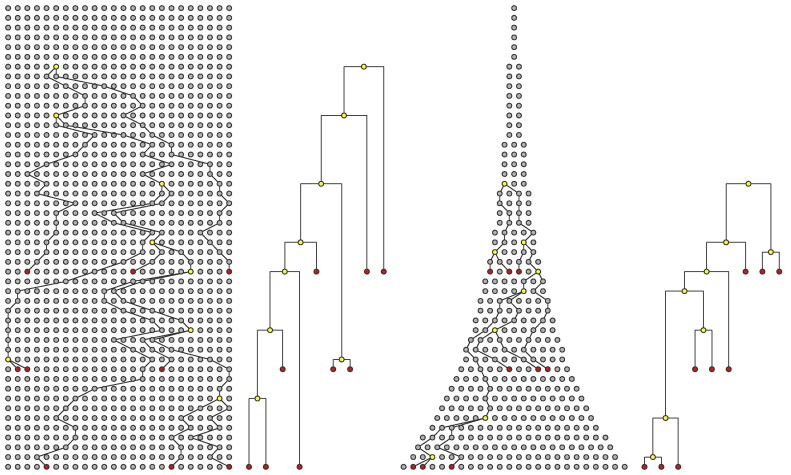
\includegraphics[scale=0.6]{figures/coalescent_serially_sampled.jpg} 
\end{figure}
\end{frame}

%-=-=-=-=-=-=-=-=-=-=-=-=-=-=-=-=-=-=-=-=-=-=-=-=
%	FRAME: time trees
%-=-=-=-=-=-=-=-=-=-=-=-=-=-=-=-=-=-=-=-=-=-=-=-=
\begin{frame}{Central object: time-calibrated trees}
\begin{column}{0.5\textwidth}
 \begin{figure}[!h]
\begin{center}
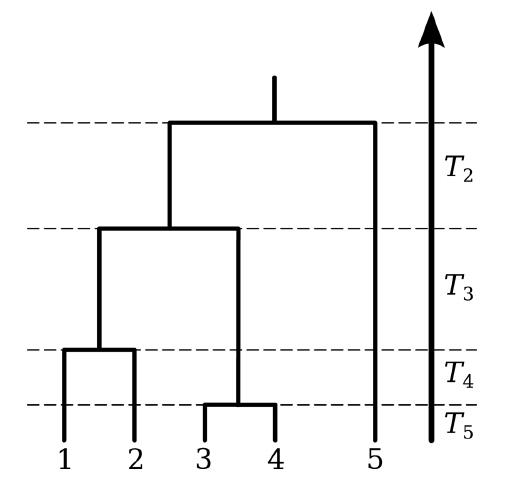
\includegraphics[scale=.45]{figures/coaltimes.jpg}
\caption{Figure 4 from Volz et al. (2013).}
\end{center}
\end{figure}
\end{column}
\begin{column}{0.45\textwidth}
{\tiny
 Let $T_n$ denote the time for $n$ lineages to~\textit{coalesce}, i.e., merge into one ancestral lineage, in a population of size $N_e$.
 Then:
\begin{align*}
Pr(T_n = t) &= \lambda_n e^{-\lambda_nt} \\
\lambda_n &= \binom{n}{2}\frac{1}{N_e} = \binom{n}{2}\frac{1}{N_e\tau}
\end{align*}
where $N_e$ is the effective population size and $\tau$ is the generation time.
Let $T_{\text{mrca}}$ denote the age of the most recent common ancestor:
\begin{align*}
 \mathbb{E}[T_{\text{mrca}}] &= \mathbb{E}[T_n] + \mathbb{E}[T_{n-1}] + \ldots + \mathbb{E}[T_2]\\
 &= 1/\lambda_n + 1/\lambda_{n-1} + \ldots + 1/\lambda_2\\
 &= 2N_e(1-\frac{1}{n})
\end{align*}
}
\end{column}
\end{frame}

%-=-=-=-=-=-=-=-=-=-=-=-=-=-=-=-=-=-=-=-=-=-=-=-=
%	FRAME: gist of BP
%-=-=-=-=-=-=-=-=-=-=-=-=-=-=-=-=-=-=-=-=-=-=-=-=
\begin{frame}{Bayesian phylogenetics}
\vspace{2em}
\begin{figure}
	\centerline{
	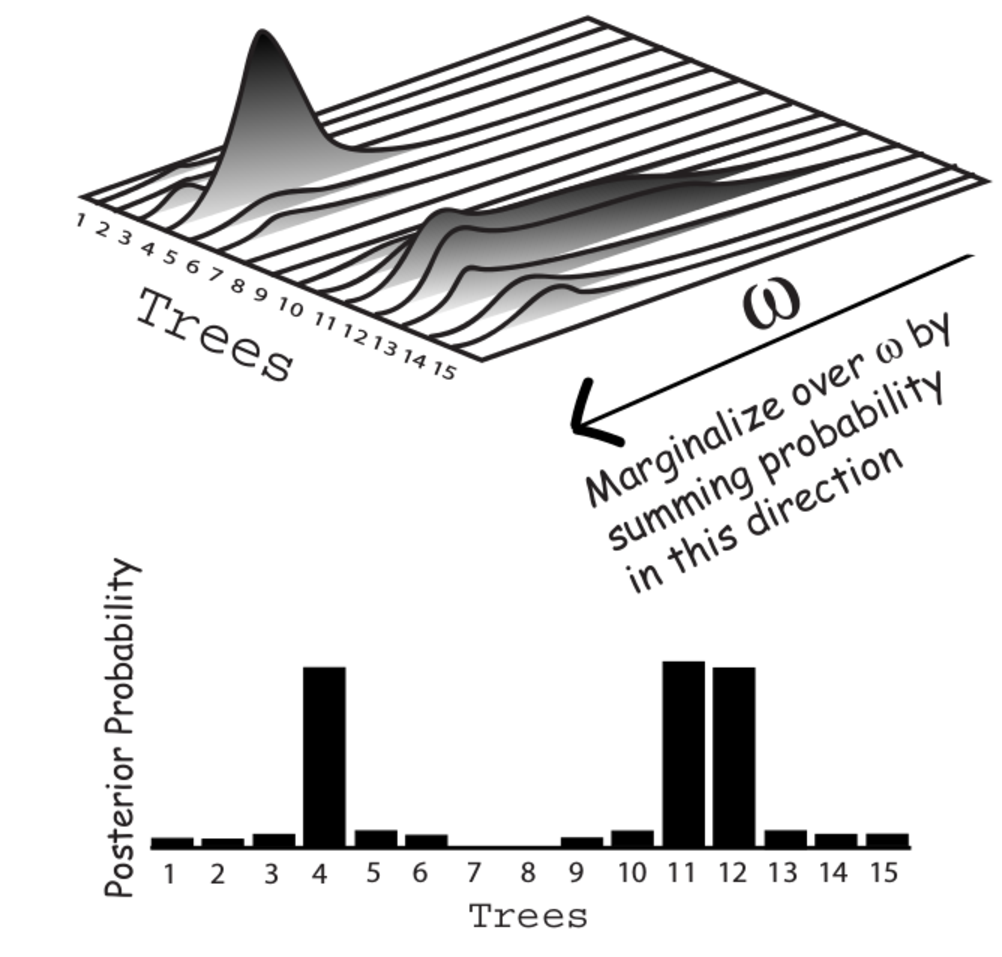
\includegraphics[width=0.55\textwidth,height=6cm]{figures/Joint_trees_omega_marg1.pdf} \\ 
	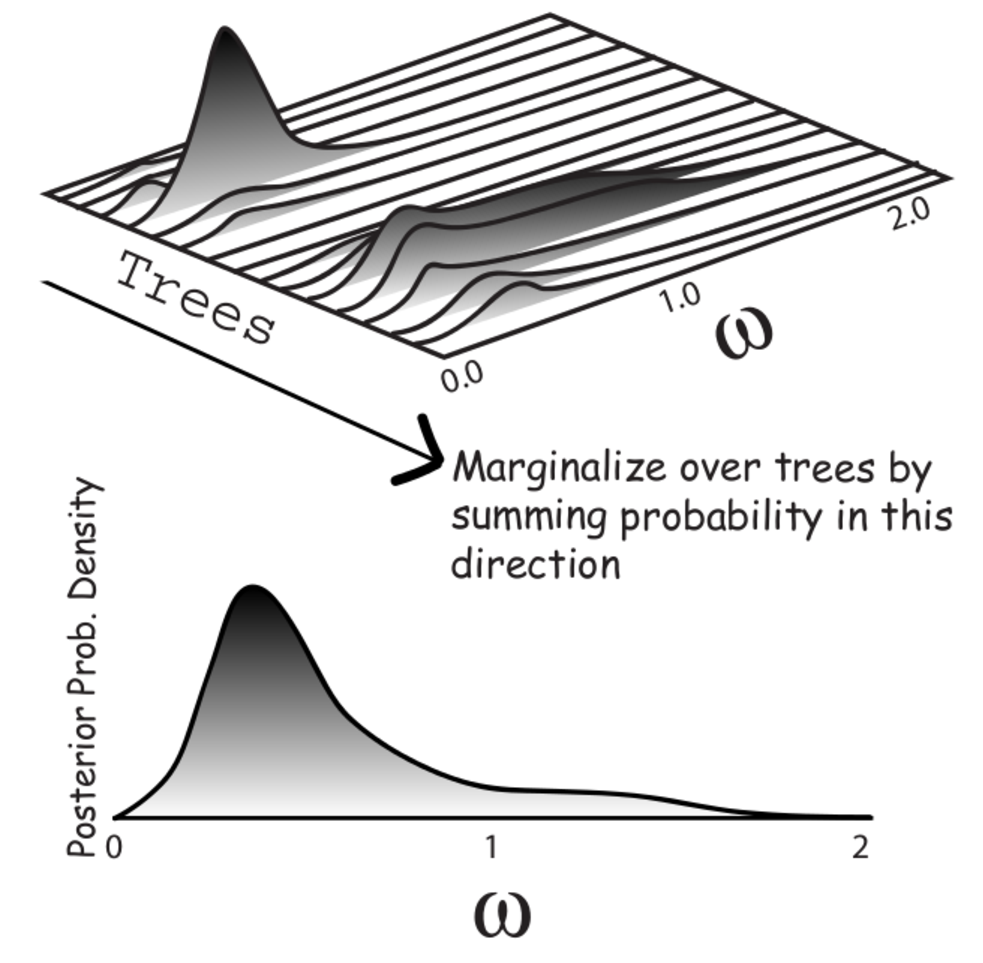
\includegraphics[width=0.55\textwidth,height=6cm]{figures/Joint_trees_omega_marg2.pdf}
	}
\end{figure}
\end{frame}

%-=-=-=-=-=-=-=-=-=-=-=-=-=-=-=-=-=-=-=-=-=-=-=-=
%	FRAME: target distribution
%-=-=-=-=-=-=-=-=-=-=-=-=-=-=-=-=-=-=-=-=-=-=-=-=
\begin{frame}{Target}
% \begin{block}{Bayesian paradigm:}
%  \textbf{Marginalise} (integrate), not maximise
% \end{block}
% \vspace{2em}
\begin{equation}
\label{eq:posterior}
 p(t, \boldsymbol b, \boldsymbol \theta | D) = \frac{f(D | t, \boldsymbol b, \boldsymbol \theta ) \pi(t, \boldsymbol b, \boldsymbol \theta )}{\sum_{t_i \in \boldsymbol T_n} \int_{\boldsymbol B}\int_{\boldsymbol \Theta} f(D | t_i, \boldsymbol b_i, \boldsymbol \theta ) \pi(t_i, \boldsymbol b_i, \boldsymbol \theta ) d\boldsymbol\theta d\boldsymbol b_i}
\end{equation}
\begin{itemize}
 \item $D$: observed data;
 \item $\boldsymbol T_n$: set of all binary ranked trees ($\mathbb{R}^{2n-2}_+ \times \mathbb{G} ^{(2n-3)!!}, $ kind of);
 \item  $\boldsymbol b_k$: set of branch lengths of $t_k \in \boldsymbol T_n$ ;
 \item $\boldsymbol \theta$: set of parameters of interest such as substitution model parameters, migration rates, heritability coefficients, etc.
\end{itemize}
\end{frame}

%-=-=-=-=-=-=-=-=-=-=-=-=-=-=-=-=-=-=-=-=-=-=-=-=
%	FRAME: Tree space
%-=-=-=-=-=-=-=-=-=-=-=-=-=-=-=-=-=-=-=-=-=-=-=-=
\begin{frame}{Tree space: a strange land}
 \begin{column}{0.55\textwidth}
\begin{figure}
	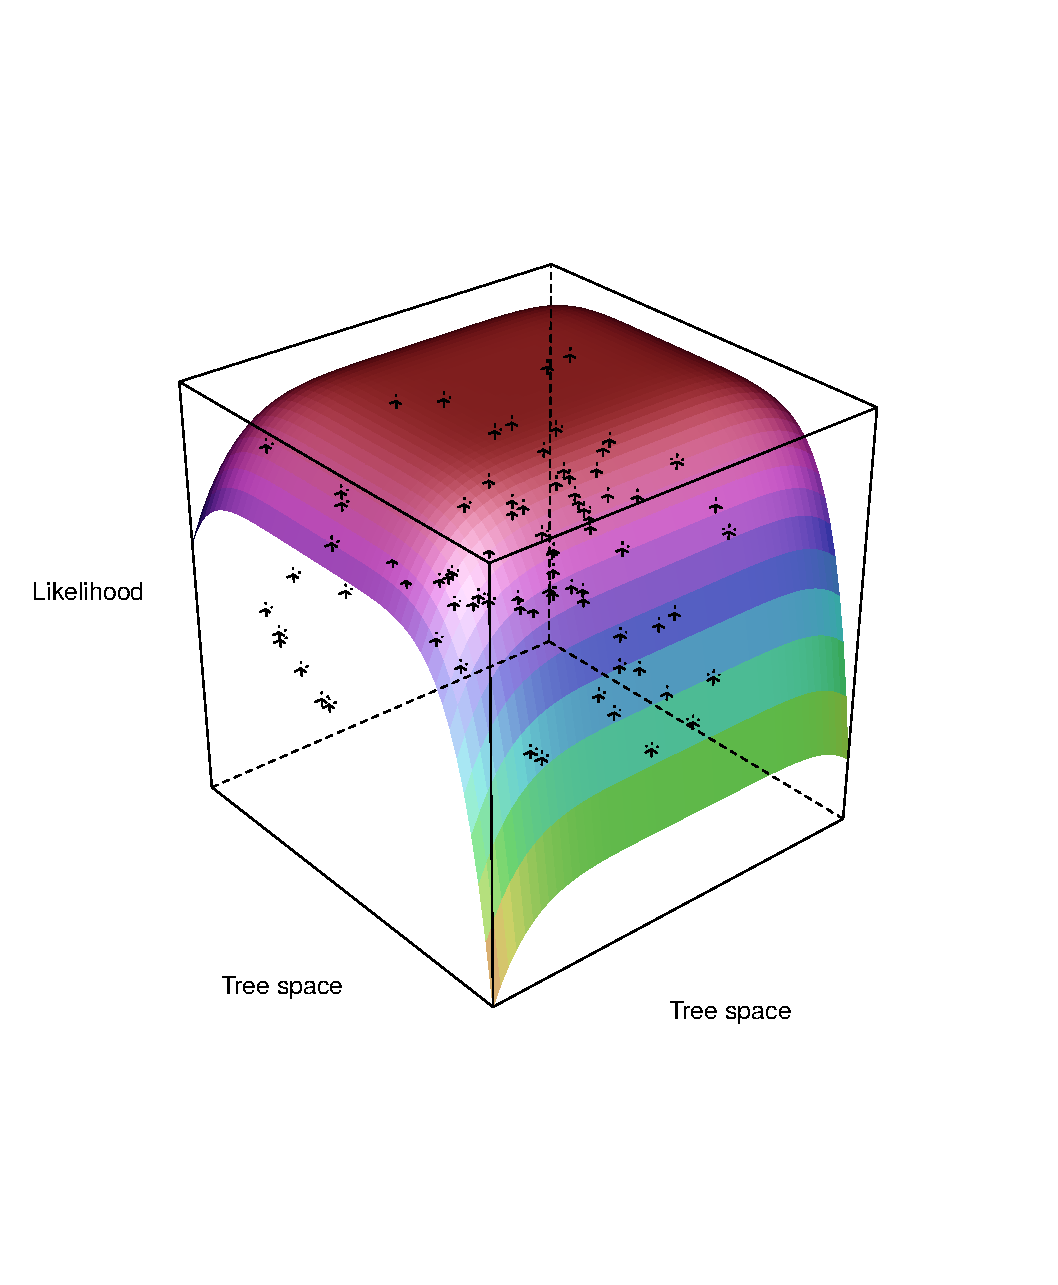
\includegraphics[width=\textwidth,height=8cm]{figures/treespace_5taxa_likelihood.pdf}
\end{figure}
\end{column}
 \begin{column}{0.45\textwidth}
\begin{figure}
	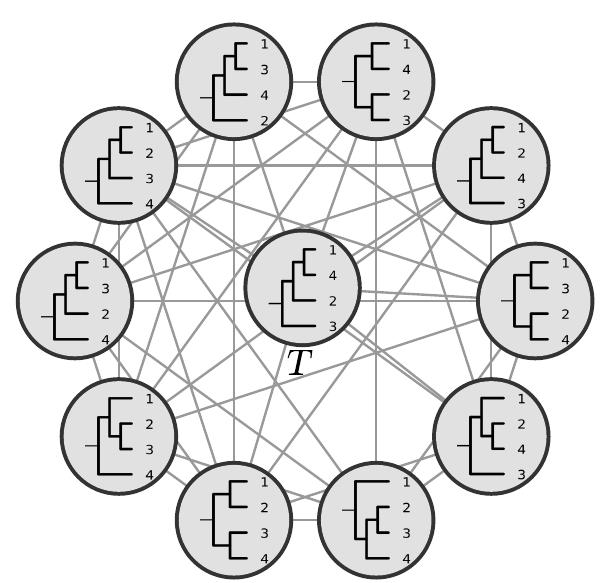
\includegraphics[width=\textwidth,height=6cm]{figures/spr_graph.jpg}
\end{figure}
\end{column}
\end{frame}

%-=-=-=-=-=-=-=-=-=-=-=-=-=-=-=-=-=-=-=-=-=-=-=-=
%	FRAME: discrete I
%-=-=-=-=-=-=-=-=-=-=-=-=-=-=-=-=-=-=-=-=-=-=-=-=
\begin{frame}{Discrete tree space: tree surgery}
\textbf{Subtree prune-and-regraft (SPR)}:
\begin{center}
 \begin{figure}
	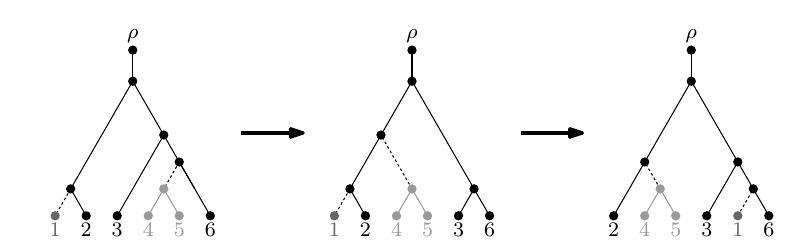
\includegraphics[scale=0.5]{figures/two_sprs.jpg}
\end{figure}
\end{center}
\end{frame}

%-=-=-=-=-=-=-=-=-=-=-=-=-=-=-=-=-=-=-=-=-=-=-=-=
%	FRAME: discrete II
%-=-=-=-=-=-=-=-=-=-=-=-=-=-=-=-=-=-=-=-=-=-=-=-=
\begin{frame}{Discrete tree space: SPR graph}
\begin{center}
 \begin{figure}
	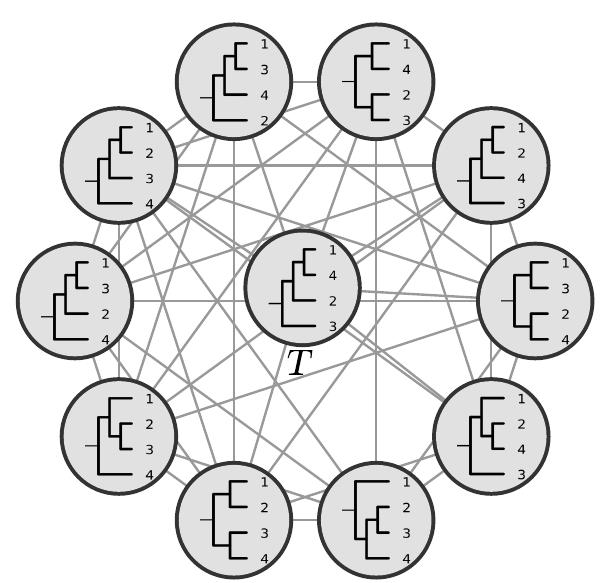
\includegraphics[scale=0.5]{figures/spr_graph.jpg}
\end{figure}
\end{center}
\end{frame}

%-=-=-=-=-=-=-=-=-=-=-=-=-=-=-=-=-=-=-=-=-=-=-=-=
%	FRAME: continuous I
%-=-=-=-=-=-=-=-=-=-=-=-=-=-=-=-=-=-=-=-=-=-=-=-=
\begin{frame}{Continuous tree space: BHV}
% \textbf{Subtree prune-and-regraft (SPR)}:
\begin{center}
 \begin{figure}
	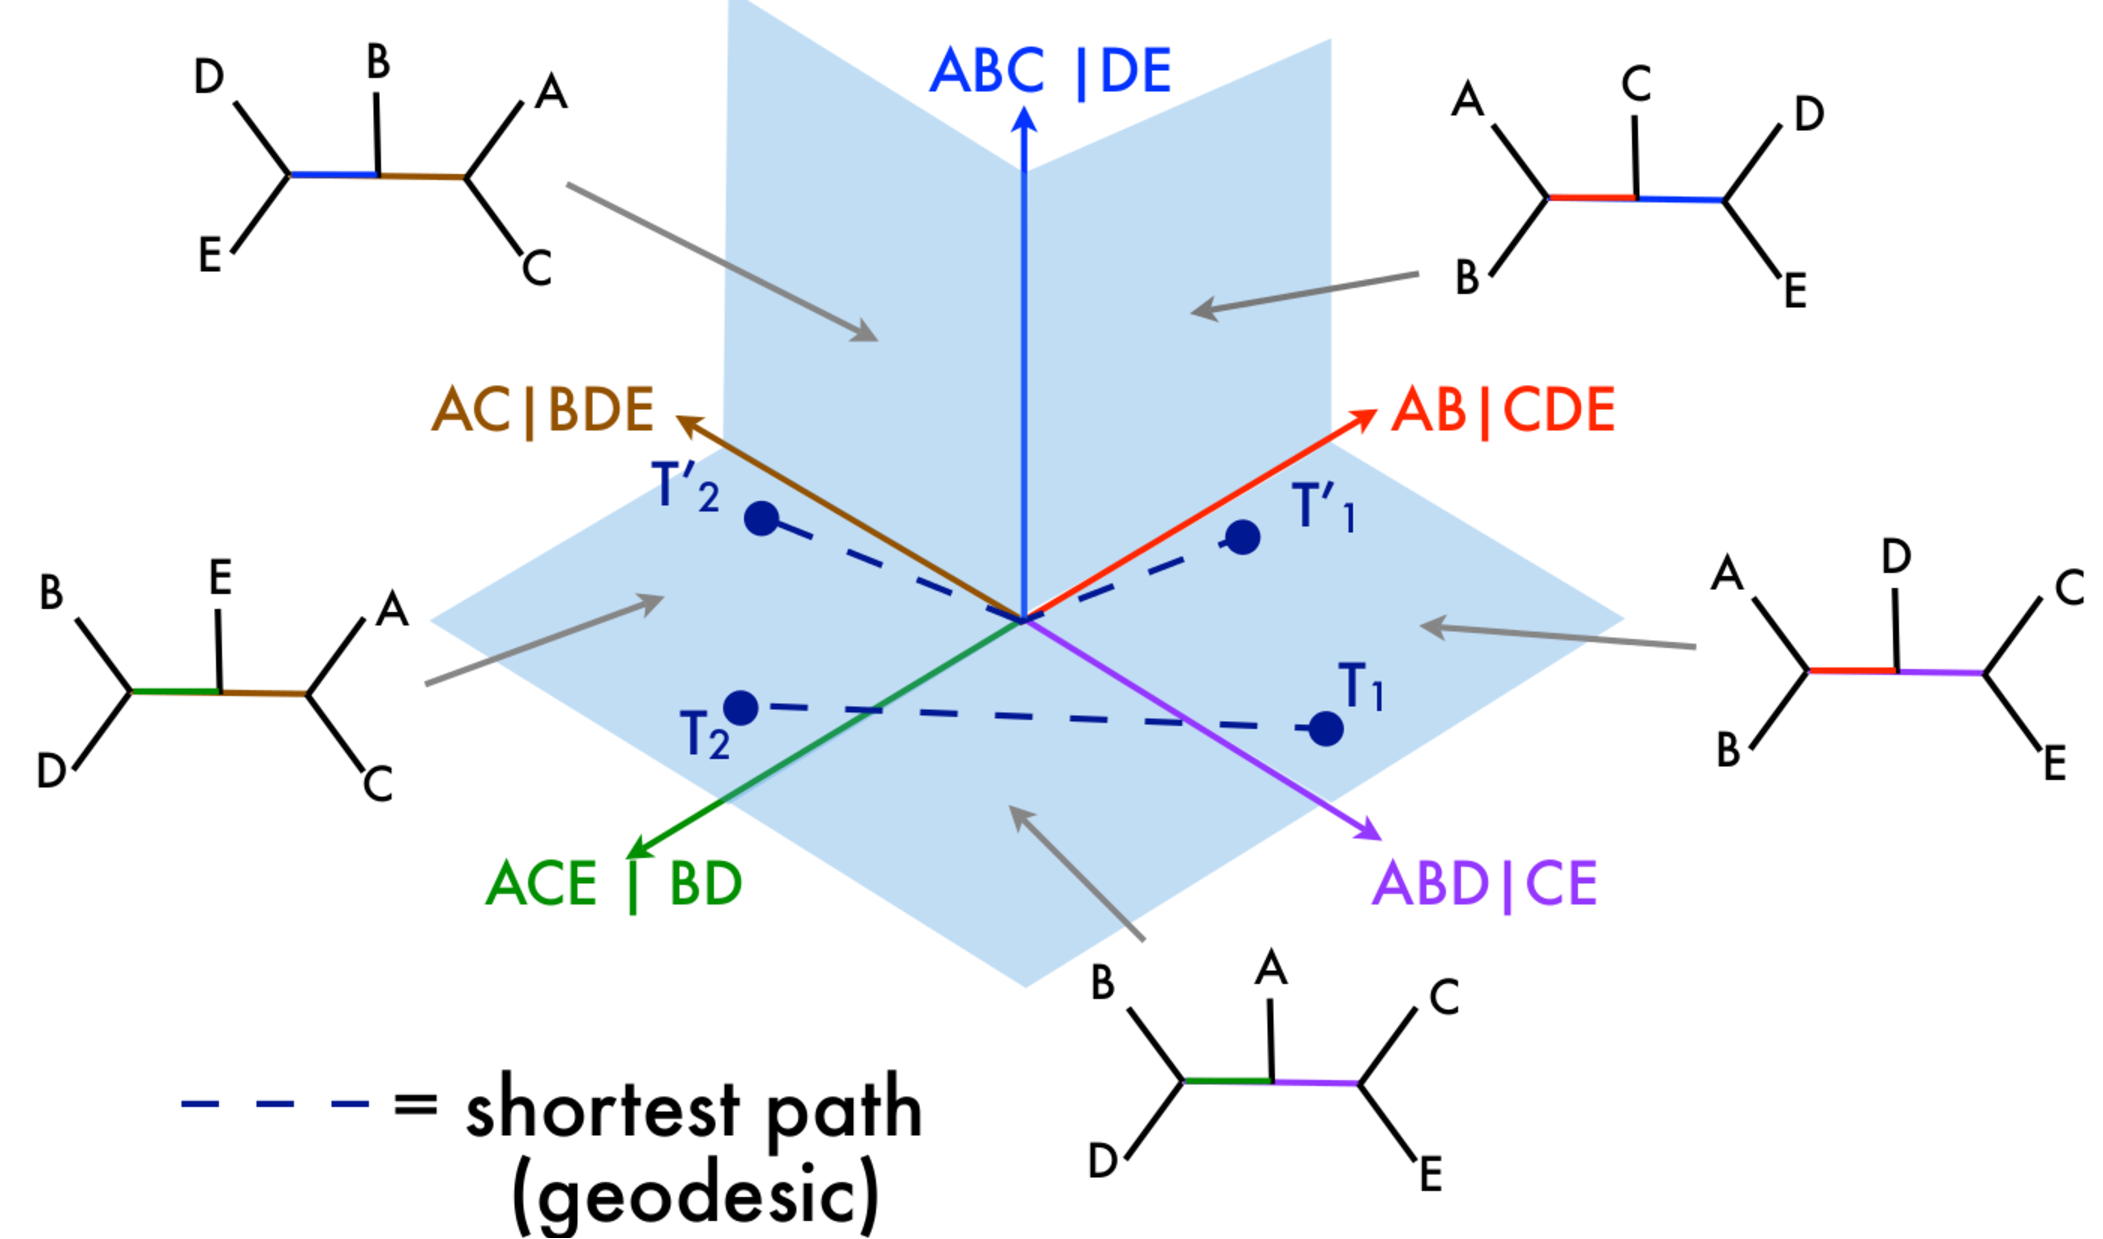
\includegraphics[scale=0.325]{figures/MeganOwen_BHV.pdf}
\end{figure}
\end{center}
\end{frame}

%-=-=-=-=-=-=-=-=-=-=-=-=-=-=-=-=-=-=-=-=-=-=-=-=
%	FRAME: Tree space MDS
%-=-=-=-=-=-=-=-=-=-=-=-=-=-=-=-=-=-=-=-=-=-=-=-=
\begin{frame}{Multi-dimensional scaling}
 \begin{column}{0.5\textwidth}
 \begin{center}
   Topology
\begin{figure}
	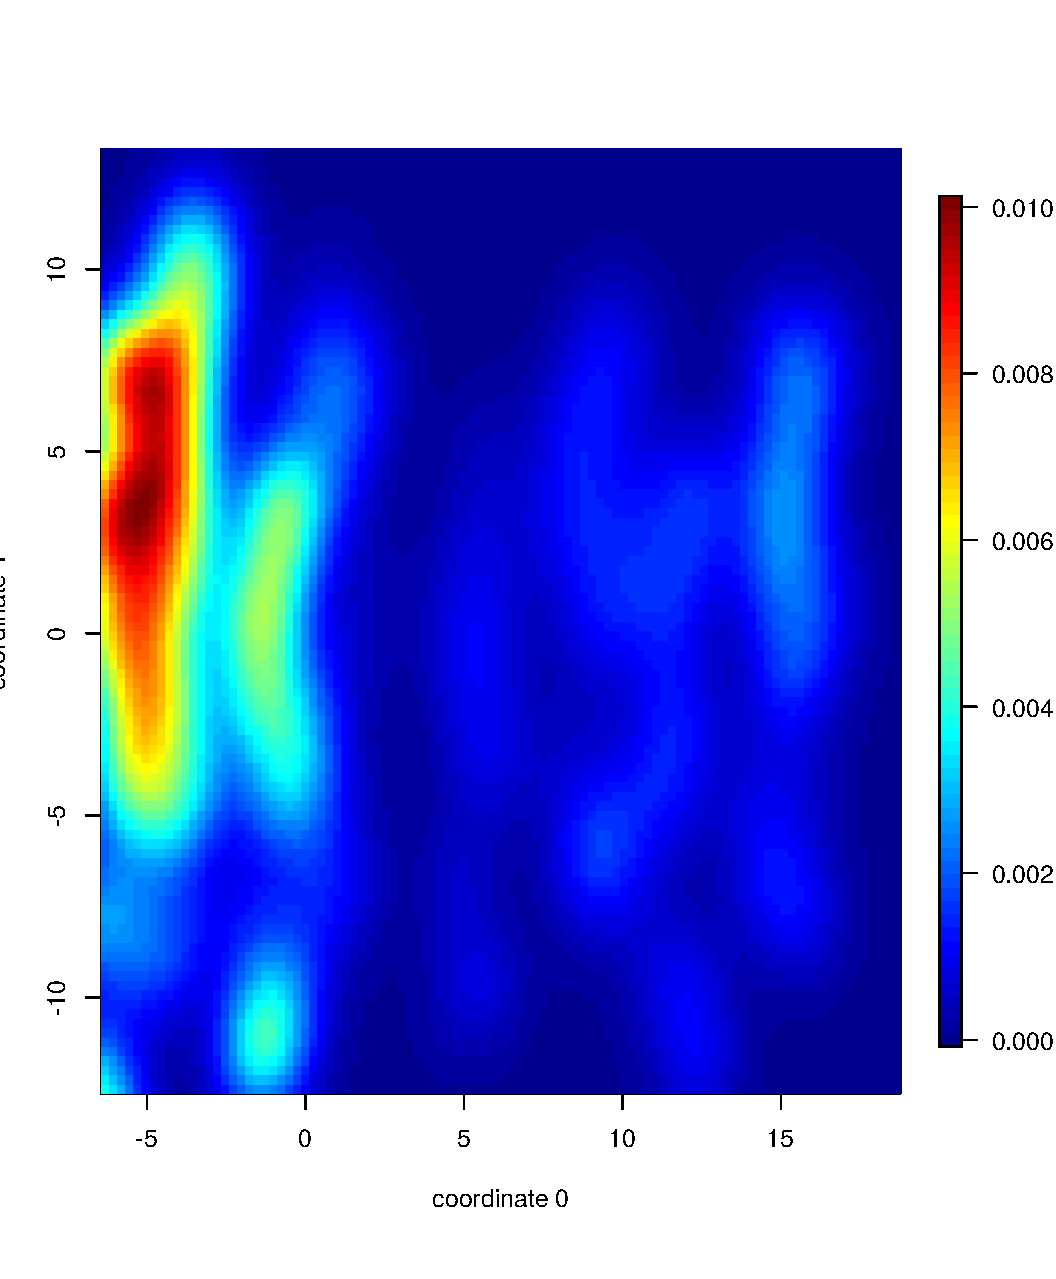
\includegraphics[width=\textwidth]{figures/RF_posterior_denv4.pdf}
\end{figure}
 \end{center}
\end{column}
 \begin{column}{0.5\textwidth}
  \begin{center}
   Topology + branches
\begin{figure}
	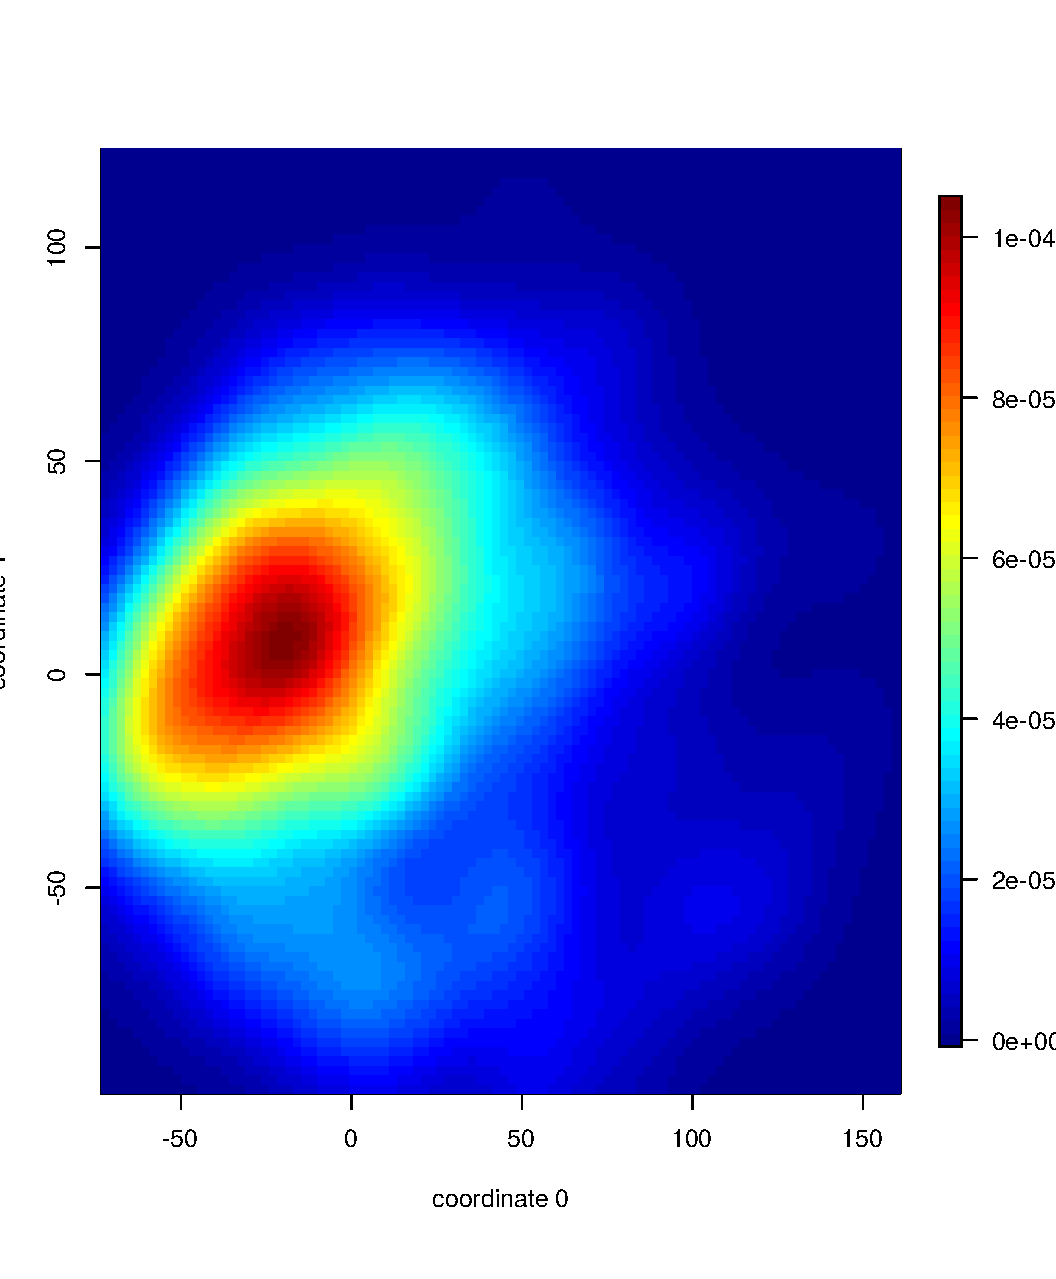
\includegraphics[width=\textwidth]{figures/BHV_posterior_denv4.pdf}
\end{figure}
 \end{center}

\end{column}
\end{frame}

%-=-=-=-=-=-=-=-=-=-=-=-=-=-=-=-=-=-=-=-=-=-=-=-=
%	FRAME: end of first half
%-=-=-=-=-=-=-=-=-=-=-=-=-=-=-=-=-=-=-=-=-=-=-=-=
\begin{frame}{Thus}
\begin{itemize}
 \item Non-standard, \textbf{huge} parameter space;
 \item No canonical representation
 \item Tip (leaf) heights impose constraints.
\end{itemize}
Open problems:
\begin{itemize}
 \item[--] Random walks on the SPR graph (and others);
 \item[--] Useful representation for time-trees;
\end{itemize}
\end{frame}

%-=-=-=-=-=-=-=-=-=-=-=-=-=-=-=-=-=-=-=-=-=-=-=-=
%	FRAME: Exploring parameter space 
%-=-=-=-=-=-=-=-=-=-=-=-=-=-=-=-=-=-=-=-=-=-=-=-=
\begin{frame}{Metropolis-Hastings for trees}

General MH setup.

Let $\tau = (t, \boldsymbol b)$ denote a tree with topology $t$ and branch lengths $\boldsymbol b$. 
For two trees $\tau$ and $\tau^\prime$, denote  the transition kernel by $q_{\gamma}(\tau| \tau^\prime) := Pr(\tau^\prime \rightarrow \tau | \gamma)$.

Accepting with probability
\[ A_{\gamma}(\tau | \tau^\prime) = min\left(1, \frac{ p(\tau^\prime, \boldsymbol \theta | D)q_{\gamma}(\tau|\tau^\prime)}{p(\tau, \boldsymbol \theta | D)q_{\gamma}(\tau^\prime|\tau)}\right) \]

leads to the desired target.

\end{frame}

%-=-=-=-=-=-=-=-=-=-=-=-=-=-=-=-=-=-=-=-=-=-=-=-=
%	FRAME: Exploring parameter space 
%-=-=-=-=-=-=-=-=-=-=-=-=-=-=-=-=-=-=-=-=-=-=-=-=
\begin{frame}{Exploring parameter space: \textbf{mixing}}
\begin{figure}
	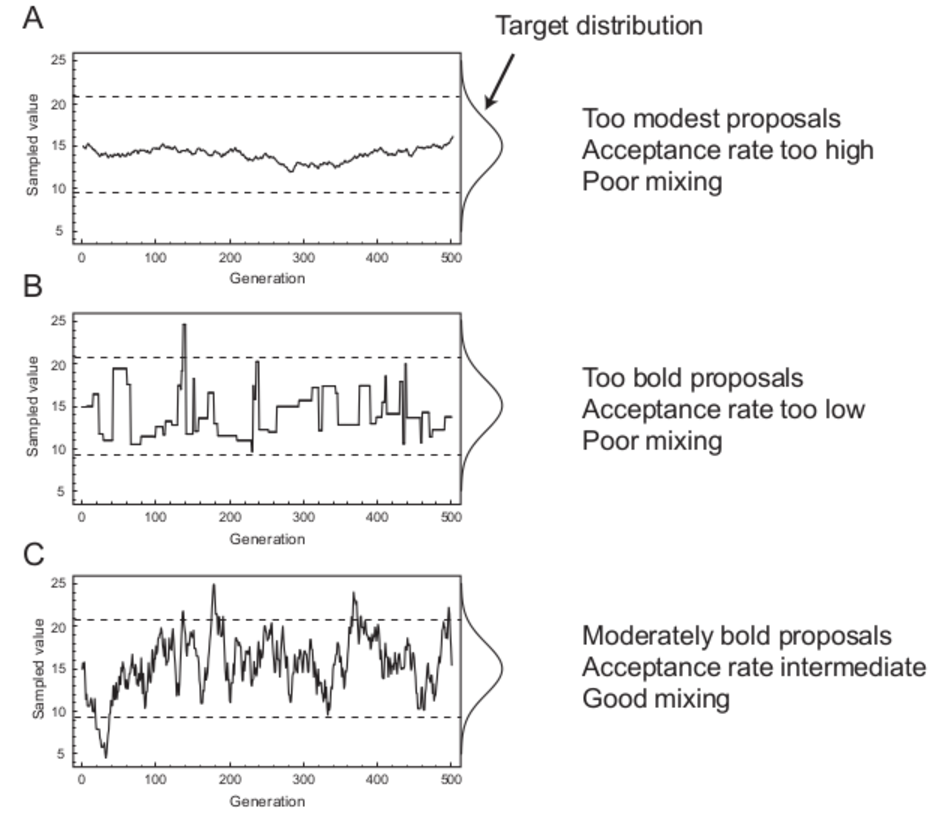
\includegraphics[width=\textwidth,height=8cm]{figures/mixing.pdf} 
\end{figure}
\end{frame}

%-=-=-=-=-=-=-=-=-=-=-=-=-=-=-=-=-=-=-=-=-=-=-=-=
%	FRAME: Time-tree kernels
%-=-=-=-=-=-=-=-=-=-=-=-=-=-=-=-=-=-=-=-=-=-=-=-=
\begin{frame}{Height-constrained kernels: SubTreeLeap}
\begin{figure}
	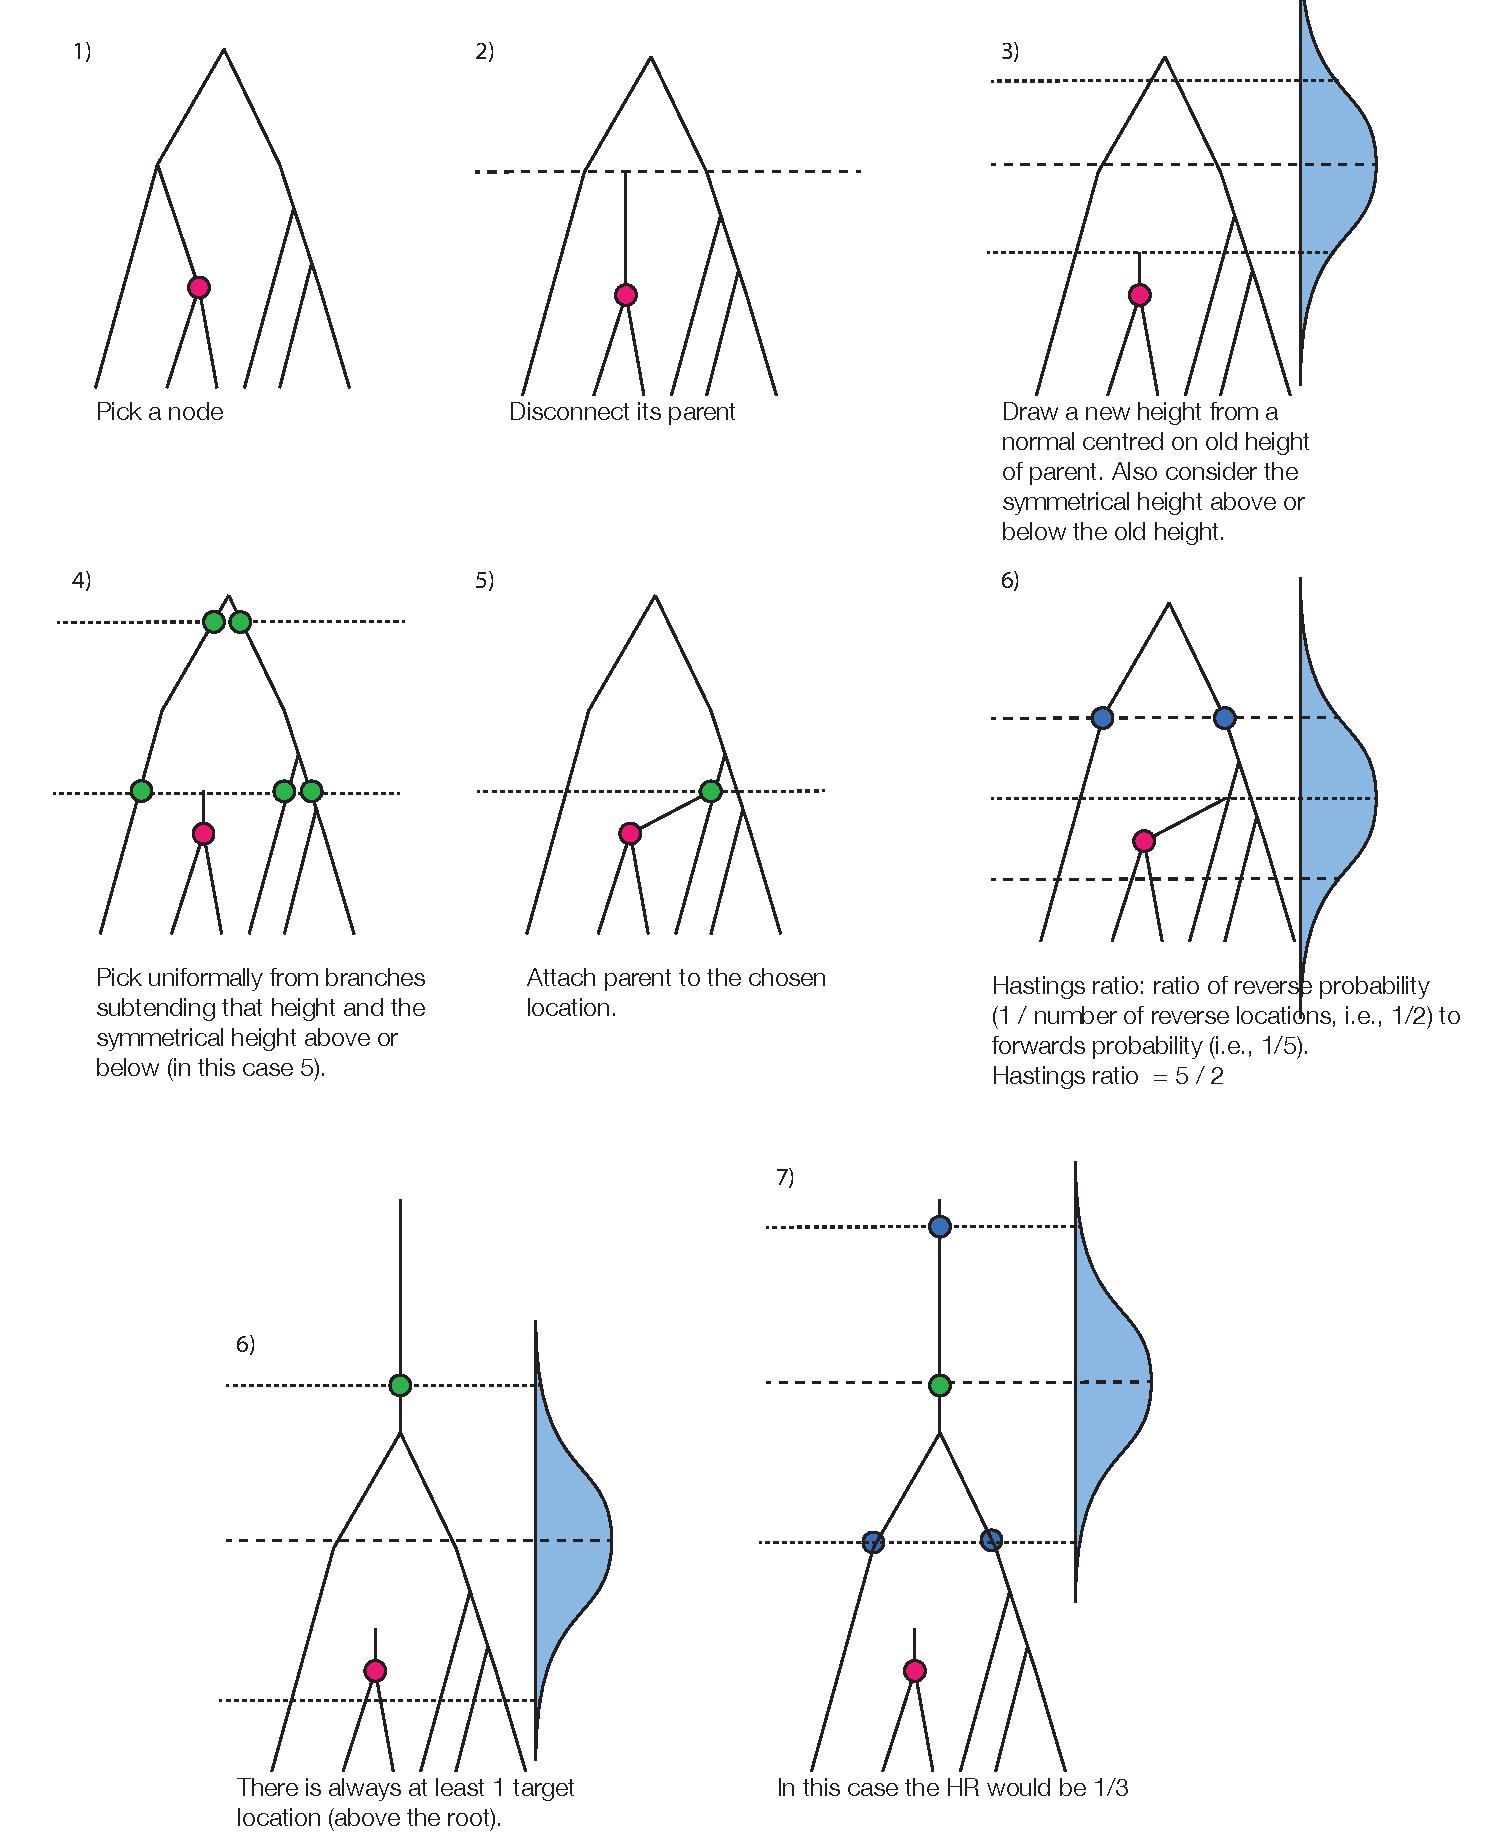
\includegraphics[width=\textwidth,height=8cm]{figures/STL_kernel.pdf} 
\end{figure}
\end{frame}

%-=-=-=-=-=-=-=-=-=-=-=-=-=-=-=-=-=-=-=-=-=-=-=-=
%	FRAME: SubTreeLeap hamiltonian
%-=-=-=-=-=-=-=-=-=-=-=-=-=-=-=-=-=-=-=-=-=-=-=-=
\begin{frame}{SubTreeLeap is Hamiltonian$^\ast$ on $\boldsymbol T_n$ }
\begin{figure}
	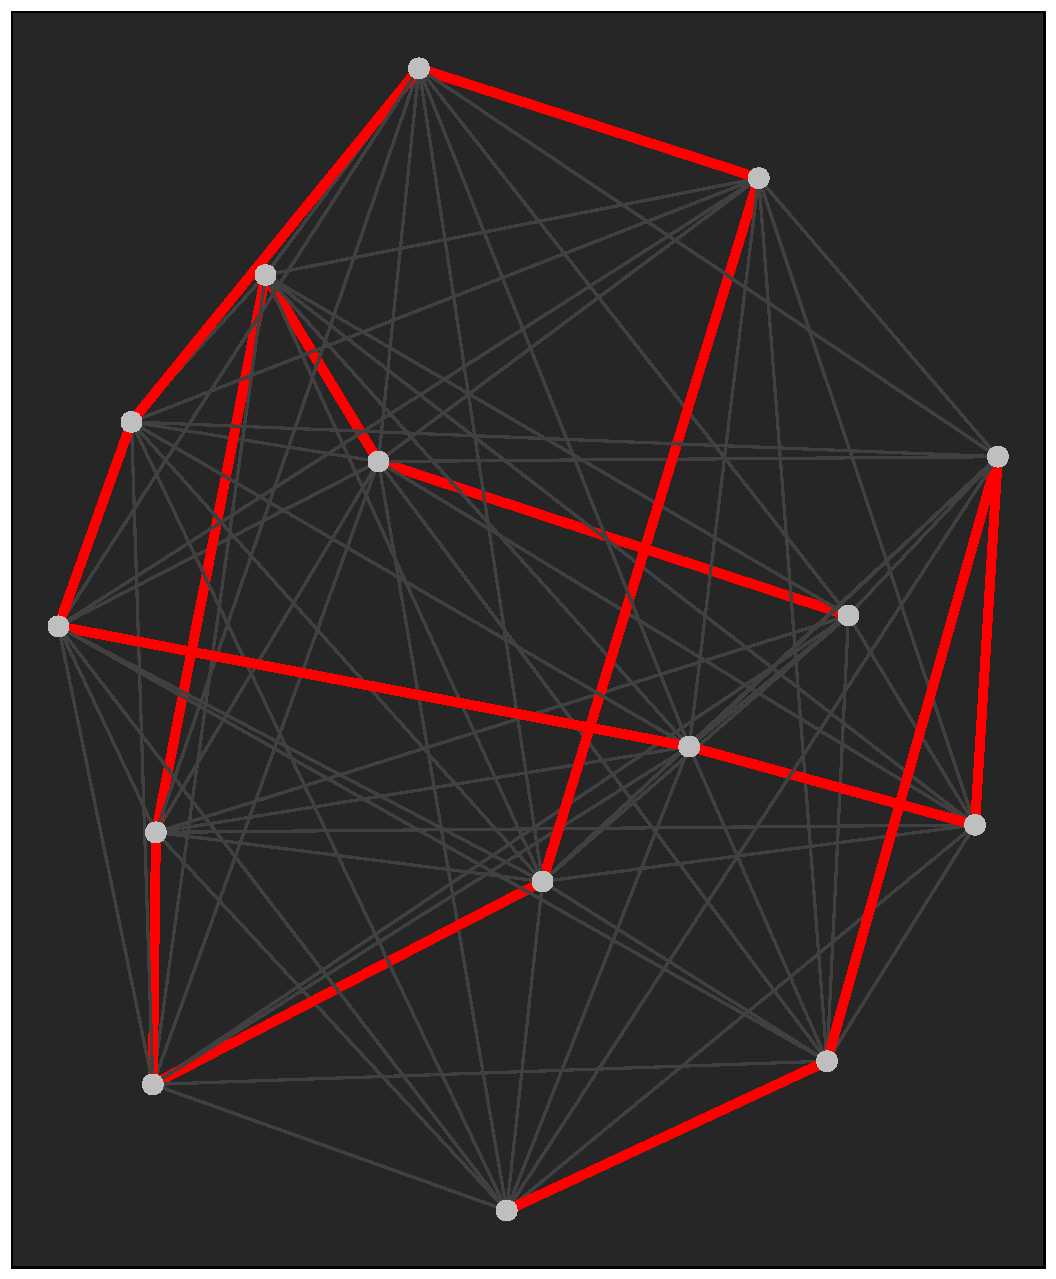
\includegraphics[scale=0.35]{figures/hamiltonian_SPR_4taxa.pdf} 
\end{figure}

\end{frame}

%-=-=-=-=-=-=-=-=-=-=-=-=-=-=-=-=-=-=-=-=-=-=-=-=
%	FRAME: Quantifying exploration of parameter space
%-=-=-=-=-=-=-=-=-=-=-=-=-=-=-=-=-=-=-=-=-=-=-=-=
\begin{frame}{Quantifying exploration}
\begin{itemize}
 \item MDS;
 \item Clade -- aka subtree -- frequencies;
 \item Clade switching;
 \item Effective sample size (ESS) of continuous parameters.
\end{itemize}
\end{frame}

%-=-=-=-=-=-=-=-=-=-=-=-=-=-=-=-=-=-=-=-=-=-=-=-=
%	FRAME: Clades: defns
%-=-=-=-=-=-=-=-=-=-=-=-=-=-=-=-=-=-=-=-=-=-=-=-=
\begin{frame}{Clade ``space''}

A clade $c$ is any collection of leaves $s_1, s_2, \ldots, s_n$ such that they share a common ancestor in the tree.
For $n$ taxa (leaves) there are $A(n) = 2^{n-1} -1$ possible clades. 

Let $\boldsymbol X_i = \{X^{(1)}, X^{(2)}, \ldots, X^{(n)}\} \in [0, 1]^n$ be a collection of samples from a Markov chain such that $X^{(j)}_i = 1$ if clade $i$ was sampled in the $j$-th iteration and $0$ otherwise.
Also, for $s_i = \sum_k X_i^{(k)}$ we call $f_i^c = s_i/n$ the \textit{frequency} of clade $i$.

\end{frame}

%-=-=-=-=-=-=-=-=-=-=-=-=-=-=-=-=-=-=-=-=-=-=-=-=
%	FRAME: Clades: frequencies
%-=-=-=-=-=-=-=-=-=-=-=-=-=-=-=-=-=-=-=-=-=-=-=-=
\begin{frame}{Clade frequencies -- deviation}

\[ \delta := \max_{1 \leq i \leq A(n)} \frac{|f^c_i - r^c_i|}{r^c_i}, \]
where $\boldsymbol f^c$ and $\boldsymbol r^c$ are the observed and true clade frequencies.

\begin{figure}
	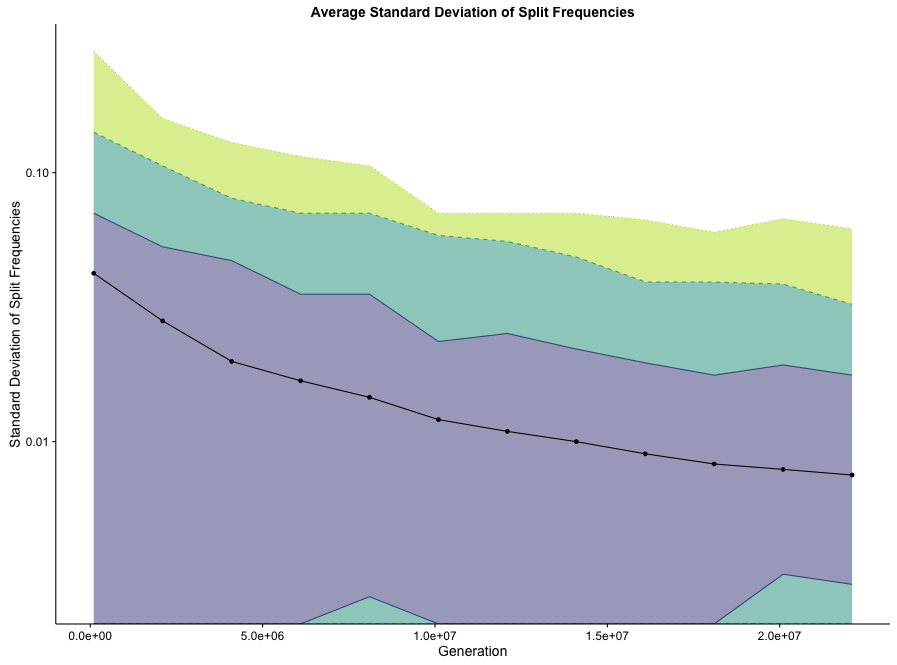
\includegraphics[scale=0.25]{figures/asdsf.png} 
\end{figure}
\end{frame}

%-=-=-=-=-=-=-=-=-=-=-=-=-=-=-=-=-=-=-=-=-=-=-=-=
%	FRAME: Clades: flipping
%-=-=-=-=-=-=-=-=-=-=-=-=-=-=-=-=-=-=-=-=-=-=-=-=
\begin{frame}{Clade switching}
Let $m_i = \min(n - s_i, s_i)$, it can be shown that the maximum number of transitions that can be observed from $\boldsymbol X_i$ is either $J_i = 2 m_i$.
% \footnote{Technically, $J_i$ depends on the first state $X_i^{(1)}$.
% Suppose w.l.o.g. that $m_i = s_i$.
% Then $J_i = 2 m_i - 1$ if $X_i^{(1)} = 1$ and $J_i = 2 m_i$ otherwise.}.

Let $\delta_i = \Delta(\boldsymbol X_i)$, where $\Delta(\cdot)$ a function that counts the number of state transitions in $\boldsymbol X_i$.
Then $\sigma_i = \delta_i/J_i \in [0, 1]$ is a score that measures the relative efficiency of sampling by comparing how how many transitions happened compared to the theoretical maximum. 
\end{frame}

%-=-=-=-=-=-=-=-=-=-=-=-=-=-=-=-=-=-=-=-=-=-=-=-=
%	FRAME: Results Denv4 MDS -- RF
%-=-=-=-=-=-=-=-=-=-=-=-=-=-=-=-=-=-=-=-=-=-=-=-=
\begin{frame}{Traversing tree space -- Topology}
 \begin{column}{0.5\textwidth}
 \begin{center}
   Default kernels
\begin{figure}
	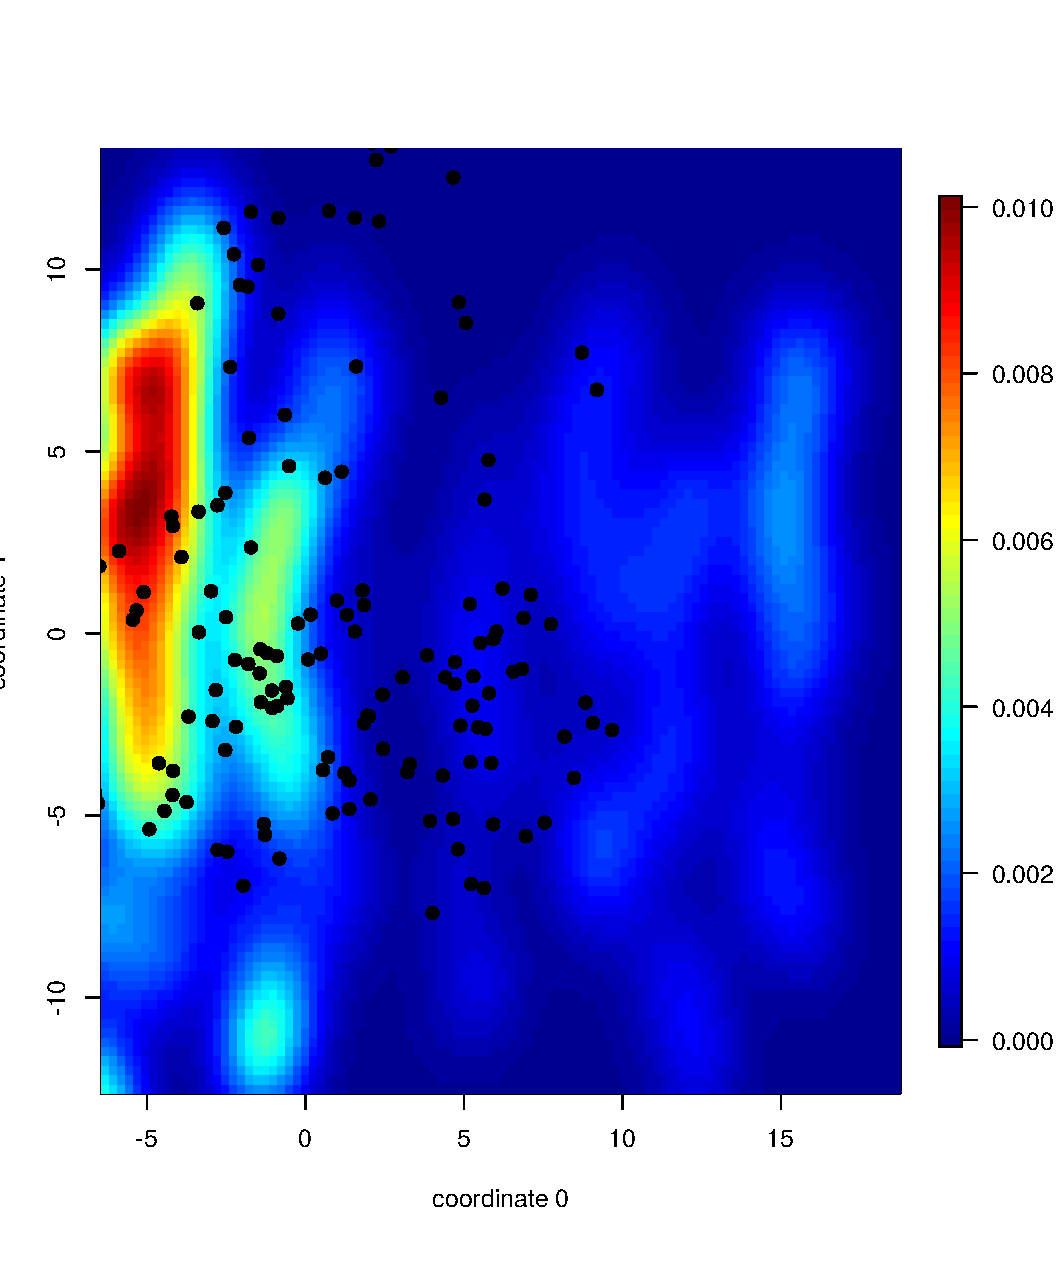
\includegraphics[width=\textwidth]{figures/mds_RF_default_denv4.pdf}
\end{figure}
 \end{center}
\end{column}
 \begin{column}{0.5\textwidth}
  \begin{center}
  STL
\begin{figure}
	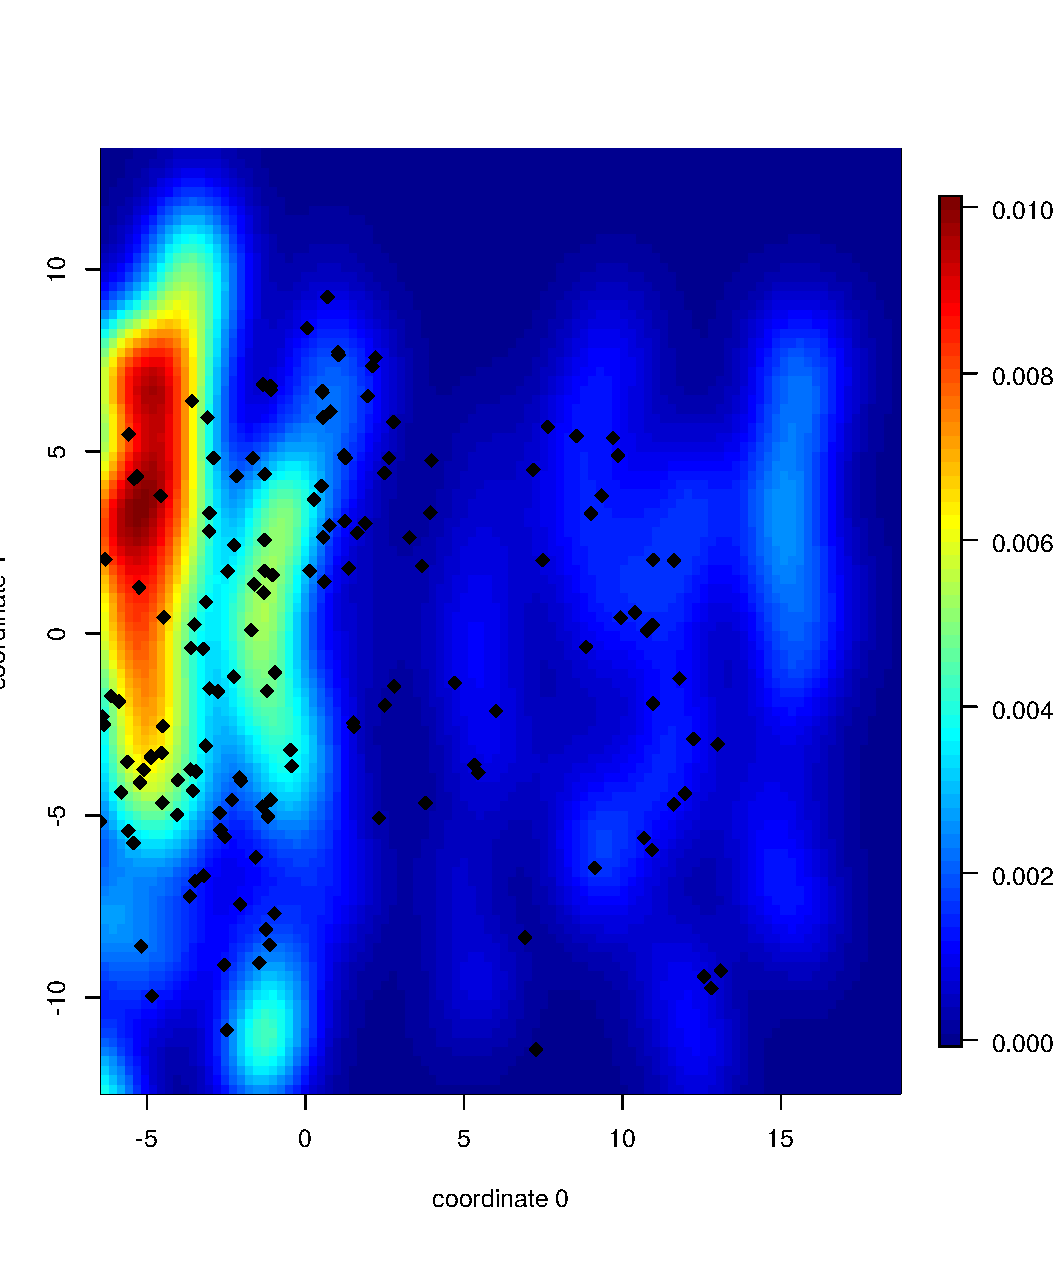
\includegraphics[width=\textwidth]{figures/mds_RF_STL_denv4.pdf}
\end{figure}
 \end{center}

\end{column}
\end{frame}

%-=-=-=-=-=-=-=-=-=-=-=-=-=-=-=-=-=-=-=-=-=-=-=-=
%	FRAME: Results Denv4 MDS -- BHV
%-=-=-=-=-=-=-=-=-=-=-=-=-=-=-=-=-=-=-=-=-=-=-=-=
\begin{frame}{Traversing tree space -- Topology + branch lengths}
 \begin{column}{0.5\textwidth}
 \begin{center}
   Default kernels
\begin{figure}
	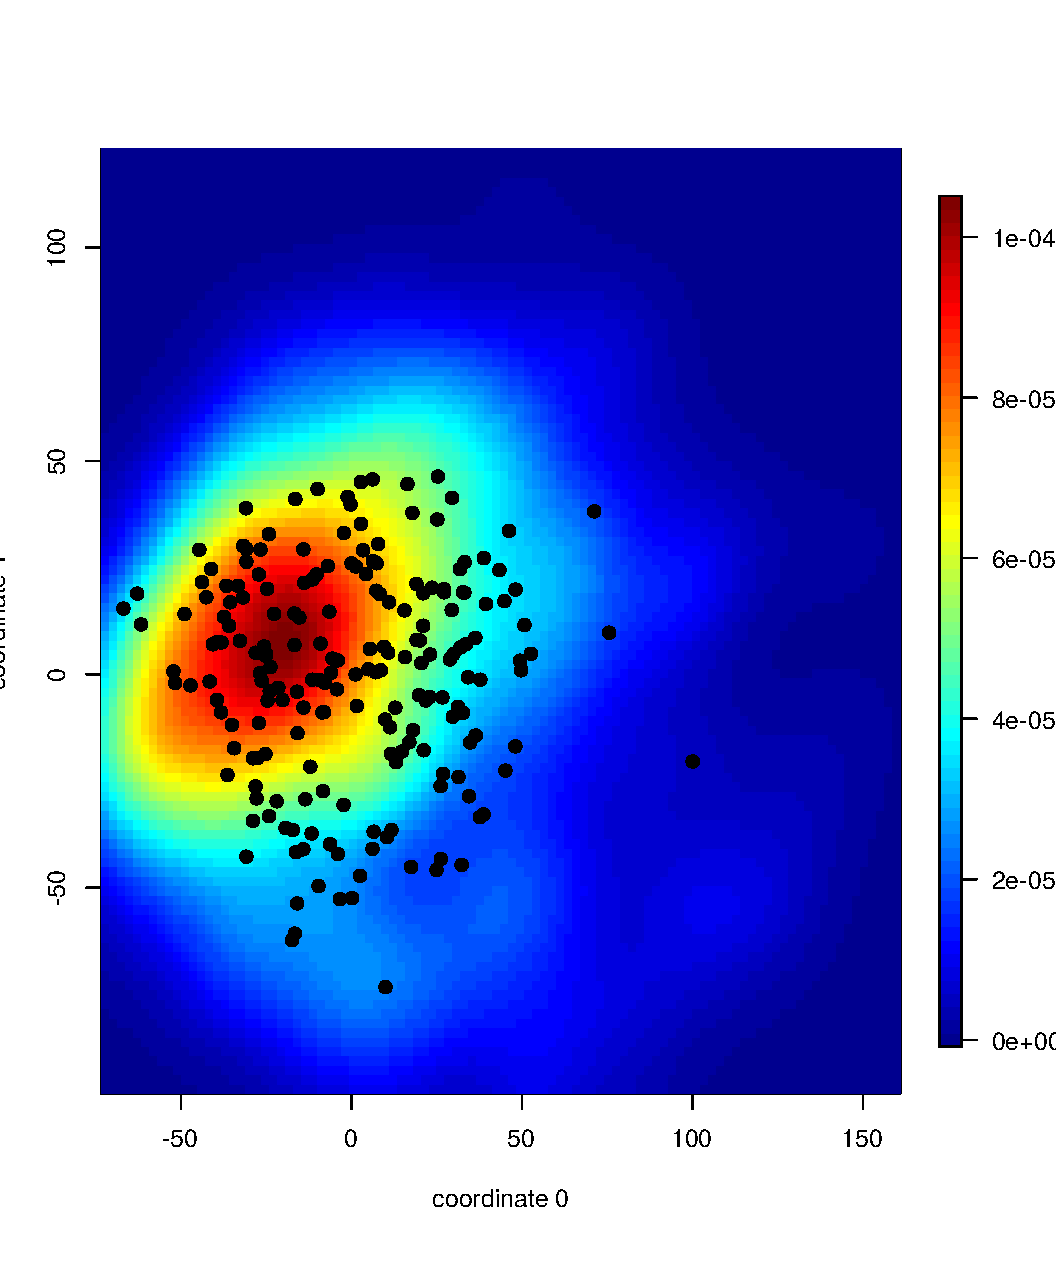
\includegraphics[width=\textwidth]{figures/mds_BHV_default_denv4.pdf}
\end{figure}
 \end{center}
\end{column}
 \begin{column}{0.5\textwidth}
  \begin{center}
  STL
\begin{figure}
	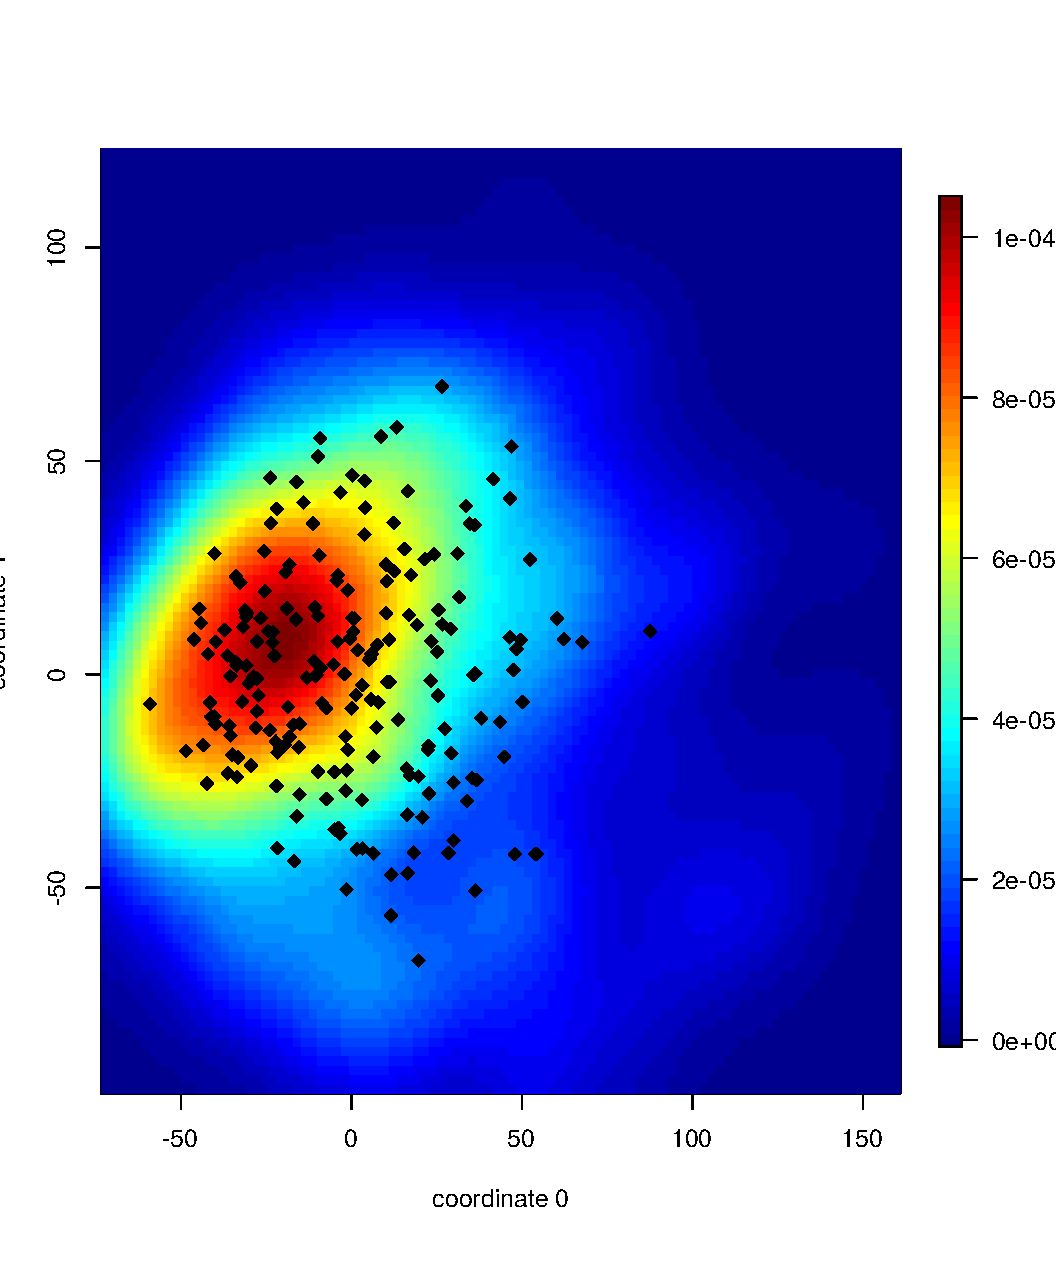
\includegraphics[width=\textwidth]{figures/mds_BHV_STL_denv4.pdf}
\end{figure}
 \end{center}

\end{column}
\end{frame}

%-=-=-=-=-=-=-=-=-=-=-=-=-=-=-=-=-=-=-=-=-=-=-=-=
%	FRAME: Results Denv4 -- clade freqs
%-=-=-=-=-=-=-=-=-=-=-=-=-=-=-=-=-=-=-=-=-=-=-=-=
\begin{frame}{Clade frequencies -- example results}
\begin{figure}
	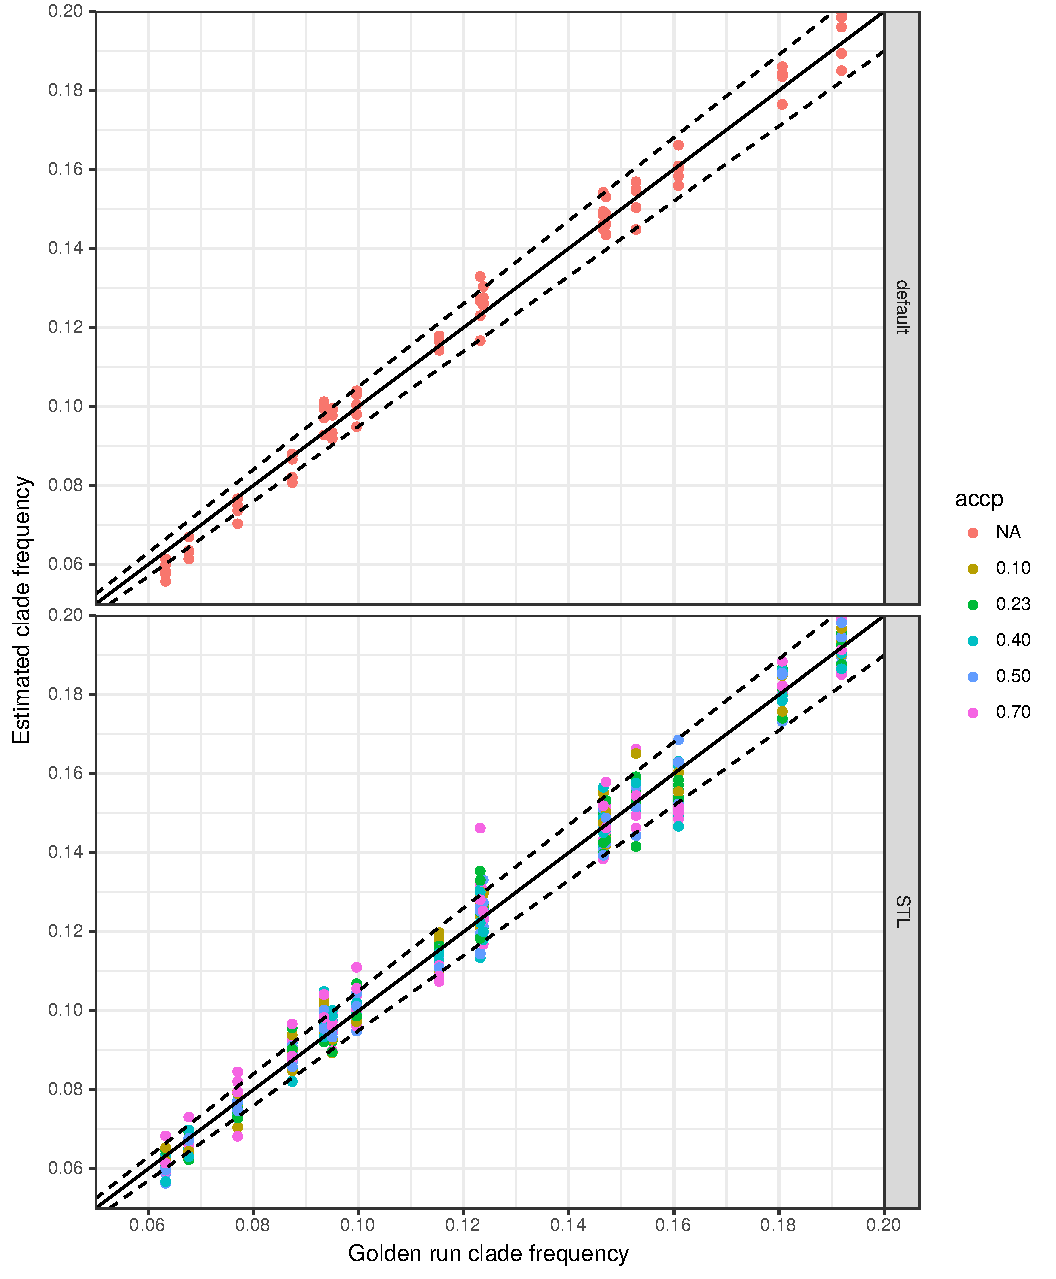
\includegraphics[scale=0.35]{figures/clade_frequencies_accP_denv17taxa.pdf} 
\end{figure}
\end{frame}

%-=-=-=-=-=-=-=-=-=-=-=-=-=-=-=-=-=-=-=-=-=-=-=-=
%	FRAME: Results Denv4 -- clade switching
%-=-=-=-=-=-=-=-=-=-=-=-=-=-=-=-=-=-=-=-=-=-=-=-=
\begin{frame}{Clade switching -- example results}
\begin{figure}
	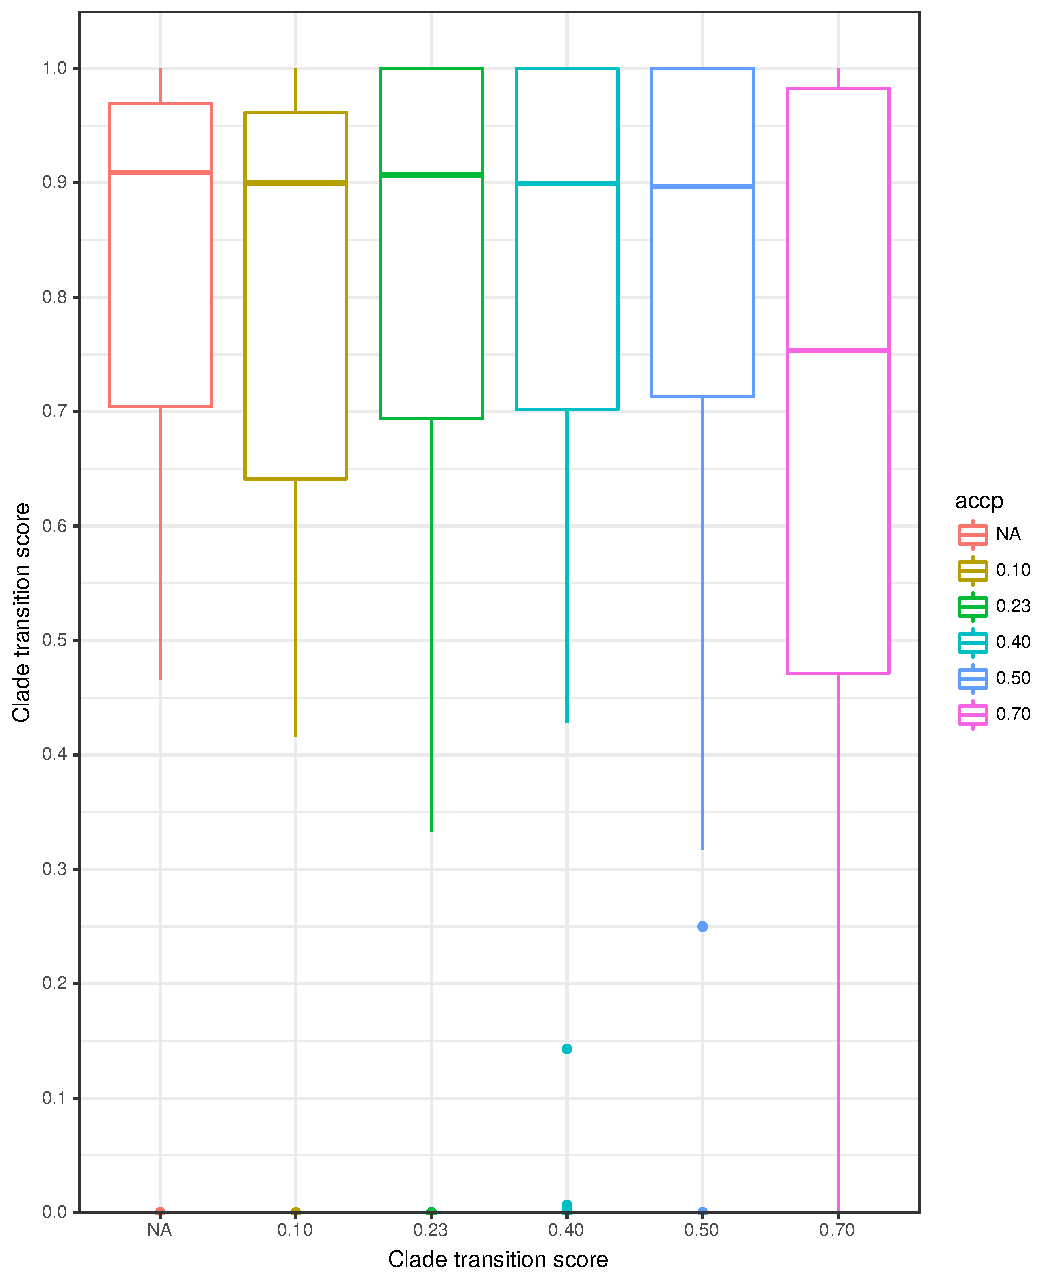
\includegraphics[scale=0.35]{figures/clade_transitions_denv17taxa.pdf} 
\end{figure}
\end{frame}

%-=-=-=-=-=-=-=-=-=-=-=-=-=-=-=-=-=-=-=-=-=-=-=-=
%	FRAME: Results Denv4
%-=-=-=-=-=-=-=-=-=-=-=-=-=-=-=-=-=-=-=-=-=-=-=-=
\begin{frame}{Dengue 4 \textit{env} (17 taxa, 1485 sites)}
\begin{figure}
\begin{column}{0.5\textwidth}
    \begin{figure}
     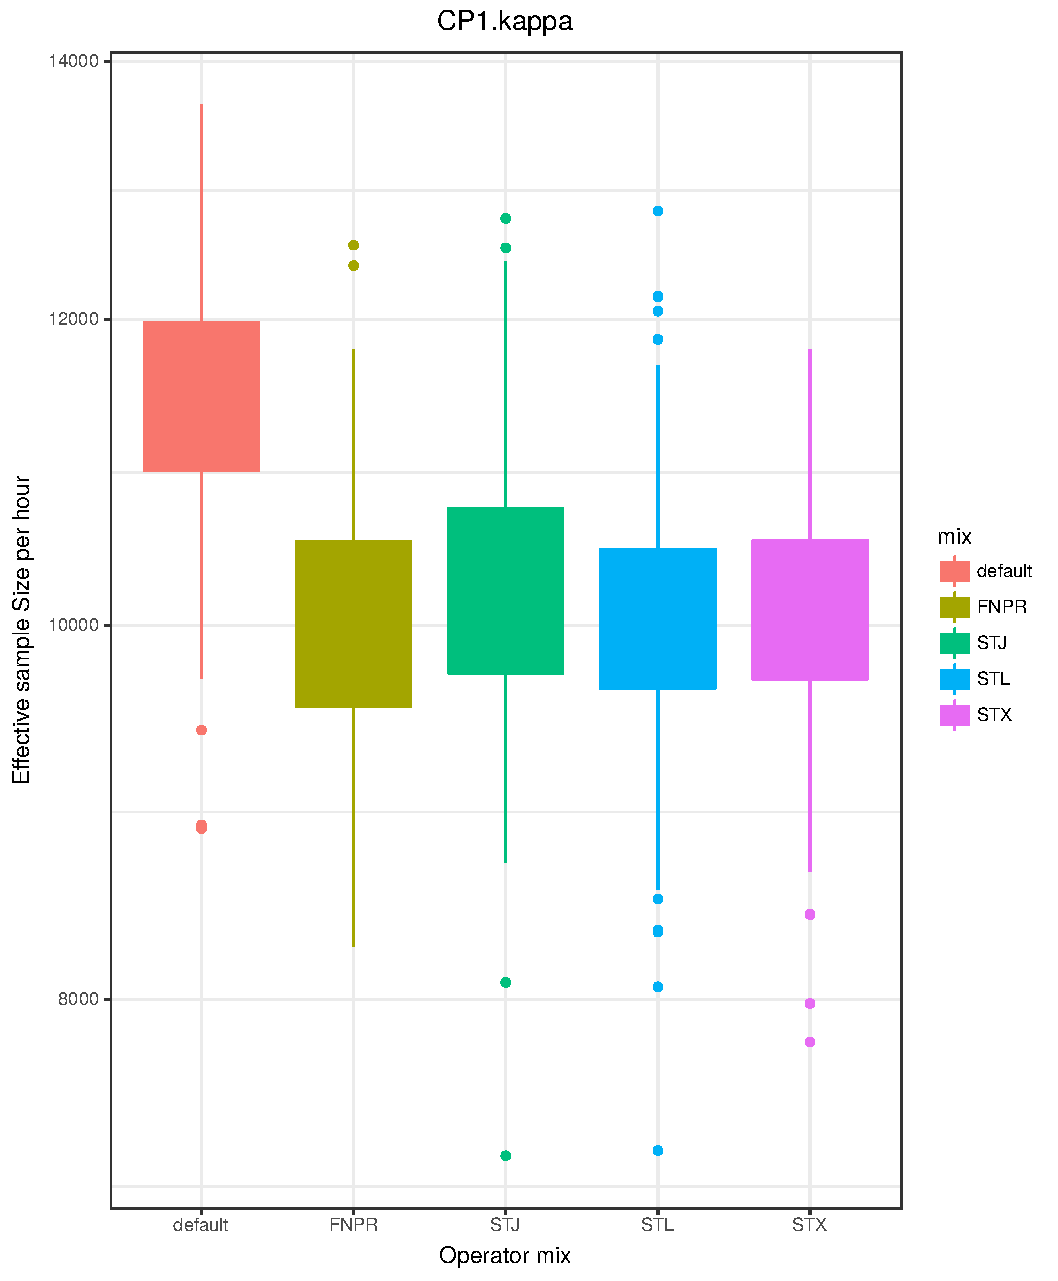
\includegraphics[width=\textwidth]{figures/ESS_hour_CP1Kappa_dengue4.pdf} \\
     \end{figure}
\end{column}
\begin{column}{0.5\textwidth}  %%<--- here
    \begin{figure}
     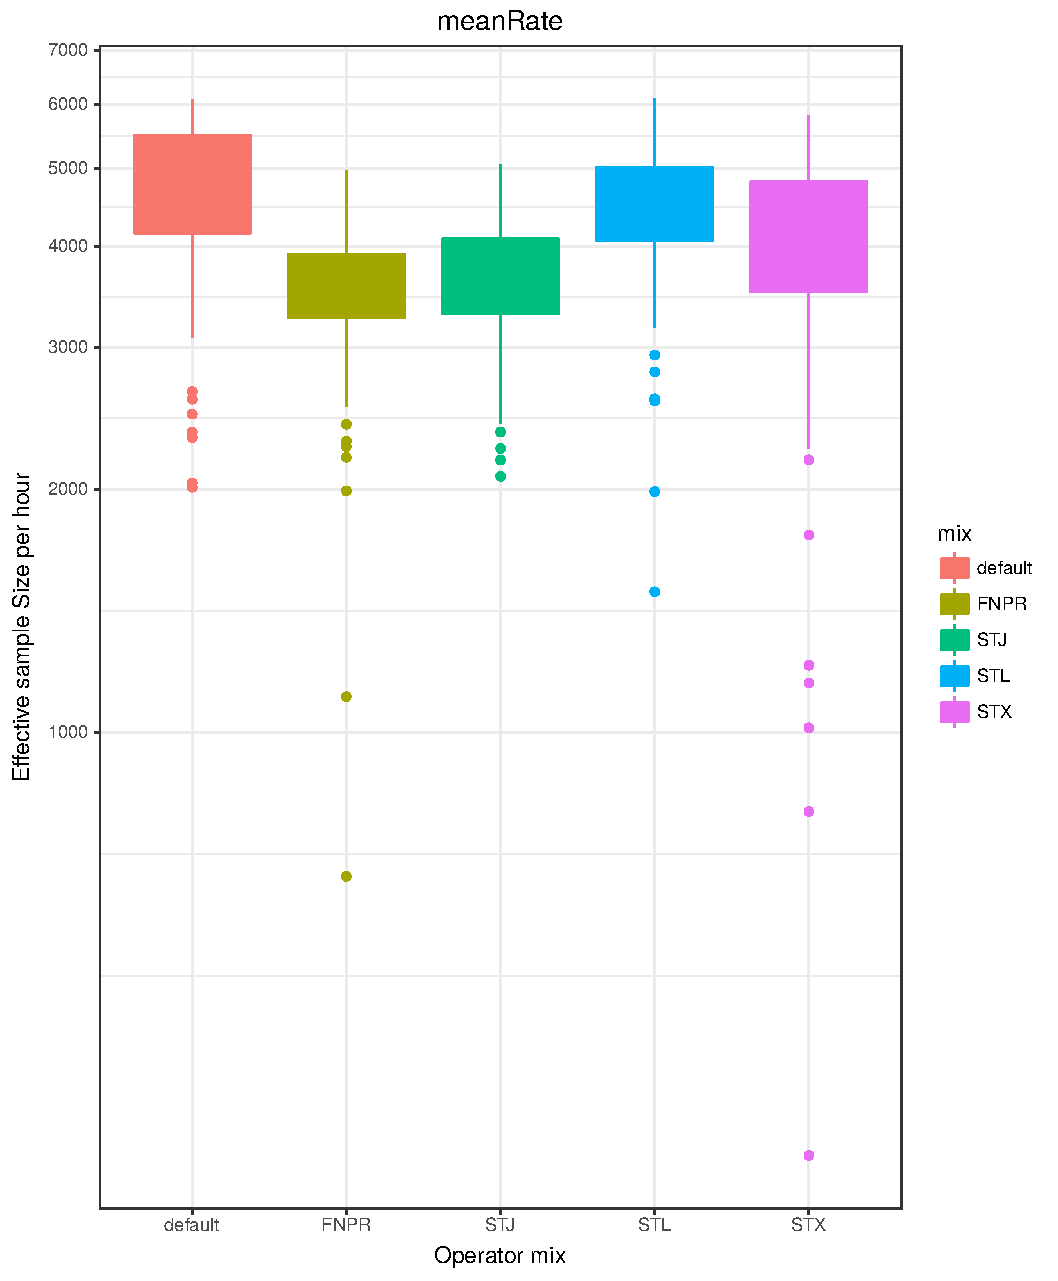
\includegraphics[width=\textwidth]{figures/ESS_hour_meanRate_dengue4.pdf} \\
     \end{figure}
\end{column}
\end{figure}
\end{frame}

%-=-=-=-=-=-=-=-=-=-=-=-=-=-=-=-=-=-=-=-=-=-=-=-=
%	FRAME: Results RSVA
%-=-=-=-=-=-=-=-=-=-=-=-=-=-=-=-=-=-=-=-=-=-=-=-=
\begin{frame}{RSVA G protein (35 taxa, 629 sites)}
\begin{figure}
\begin{column}{0.5\textwidth}
    \begin{figure}
     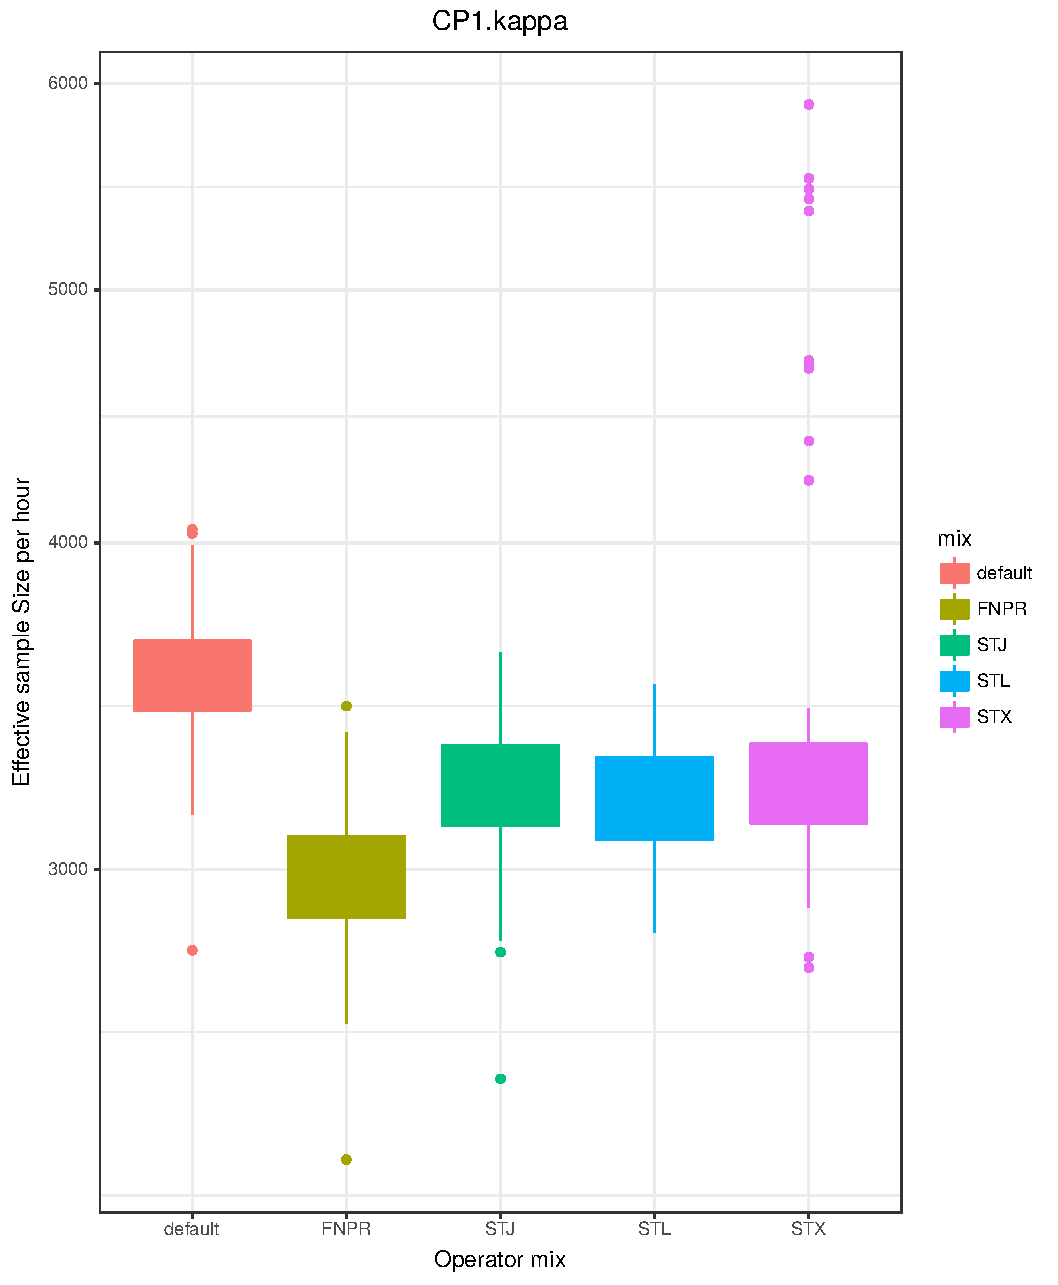
\includegraphics[width=\textwidth]{figures/ESS_hour_CP1Kappa_RSVA.pdf} \\
     \end{figure}
\end{column}
\begin{column}{0.5\textwidth}  %%<--- here
    \begin{figure}
     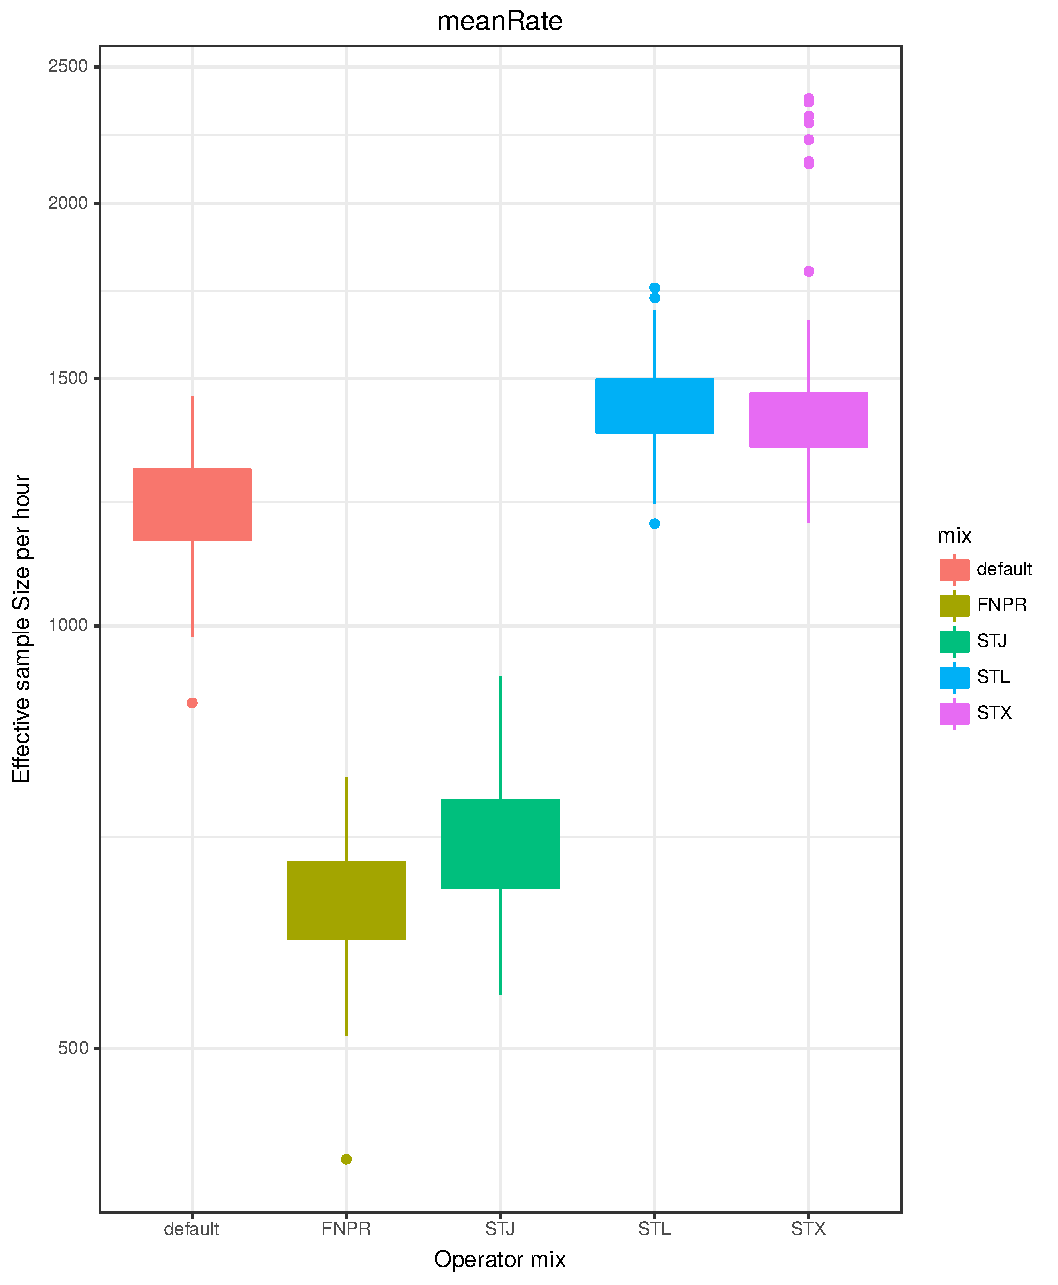
\includegraphics[width=\textwidth]{figures/ESS_hour_meanRate_RSVA.pdf} \\
     \end{figure}
\end{column}
\end{figure}
\end{frame}

%-=-=-=-=-=-=-=-=-=-=-=-=-=-=-=-=-=-=-=-=-=-=-=-=
%	FRAME: Results YFV
%-=-=-=-=-=-=-=-=-=-=-=-=-=-=-=-=-=-=-=-=-=-=-=-=
\begin{frame}{YFV \textit{prM/E} gene (71 taxa, 654 sites)}
\begin{figure}
\begin{column}{0.5\textwidth}
    \begin{figure}
     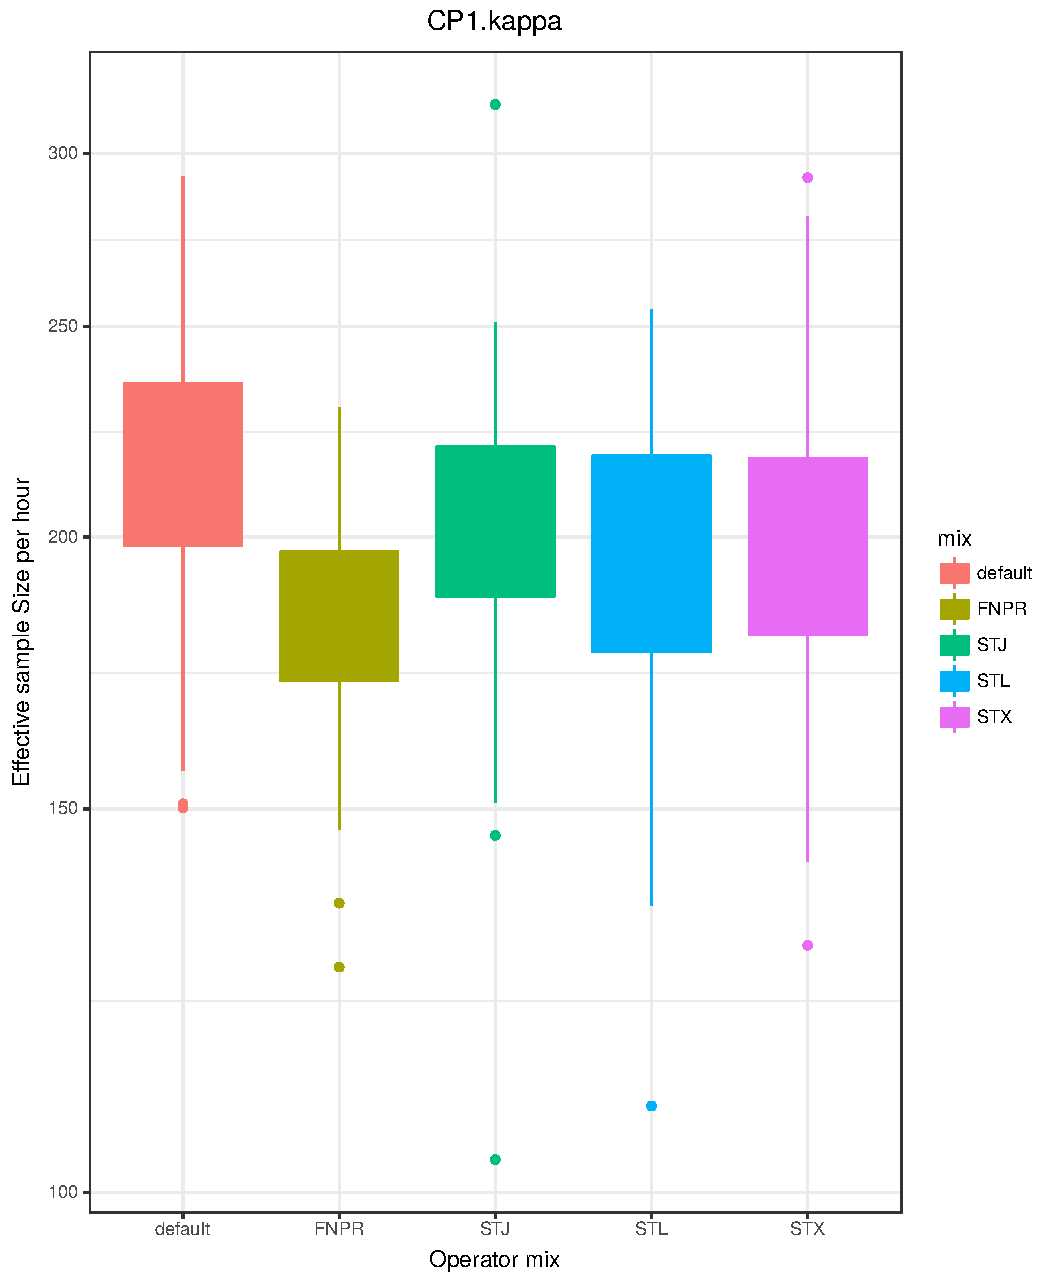
\includegraphics[width=\textwidth]{figures/ESS_hour_CP1Kappa_YFV.pdf} \\
     \end{figure}
\end{column}
\begin{column}{0.5\textwidth}  %%<--- here
    \begin{figure}
     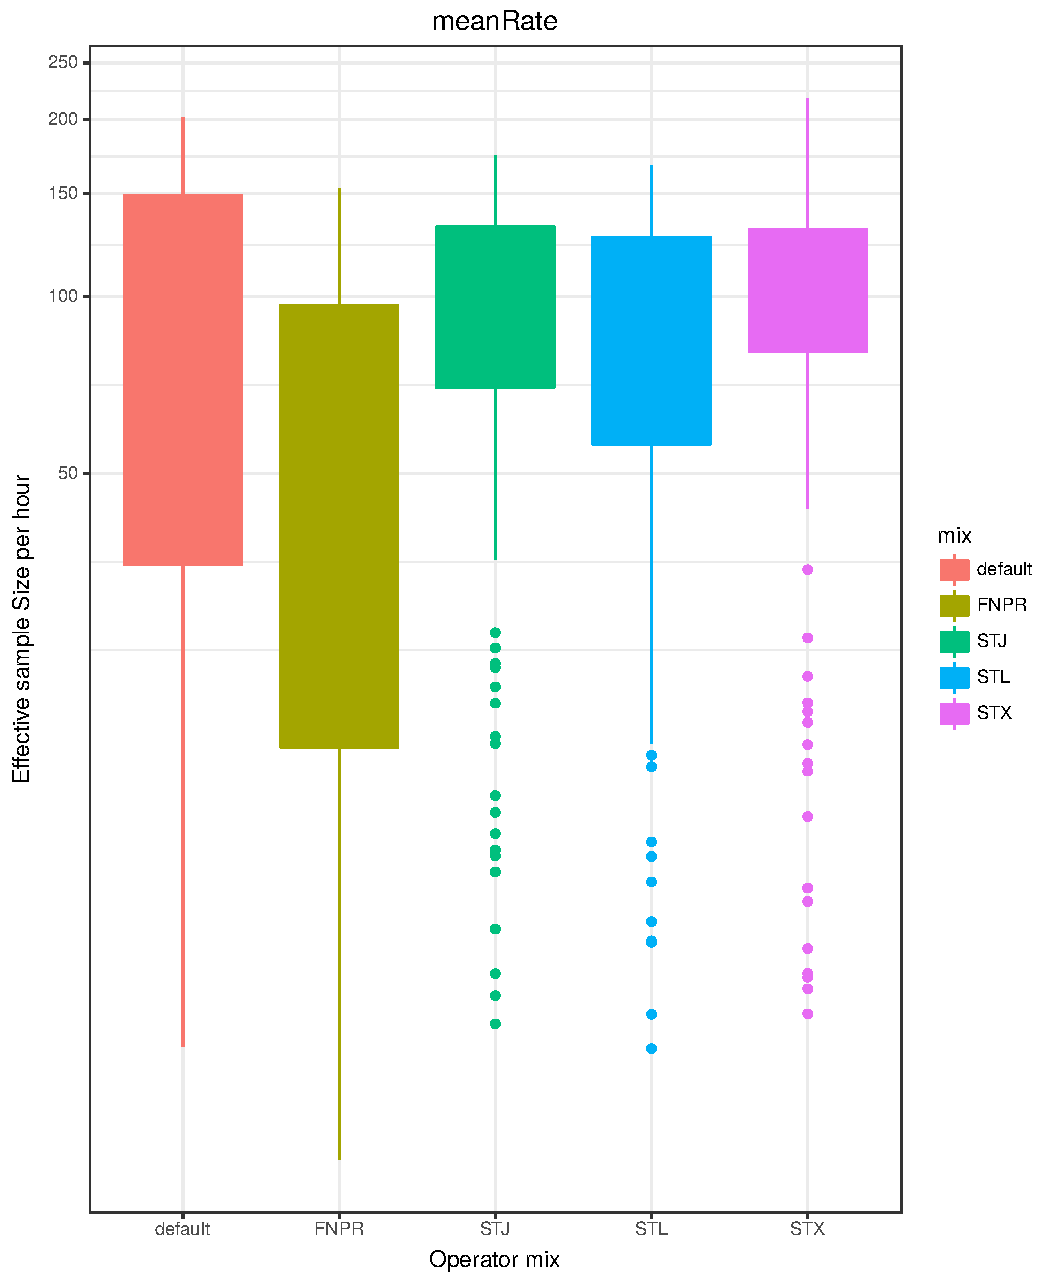
\includegraphics[width=\textwidth]{figures/ESS_hour_meanRate_YFV.pdf} \\
     \end{figure}
\end{column}
\end{figure}
\end{frame}

%-=-=-=-=-=-=-=-=-=-=-=-=-=-=-=-=-=-=-=-=-=-=-=-=
%	FRAME: Results Extra
%-=-=-=-=-=-=-=-=-=-=-=-=-=-=-=-=-=-=-=-=-=-=-=-=
\begin{frame}{Metazoans (contemporaneous, 55 taxa, 30257 AA sites)}
\begin{figure}
	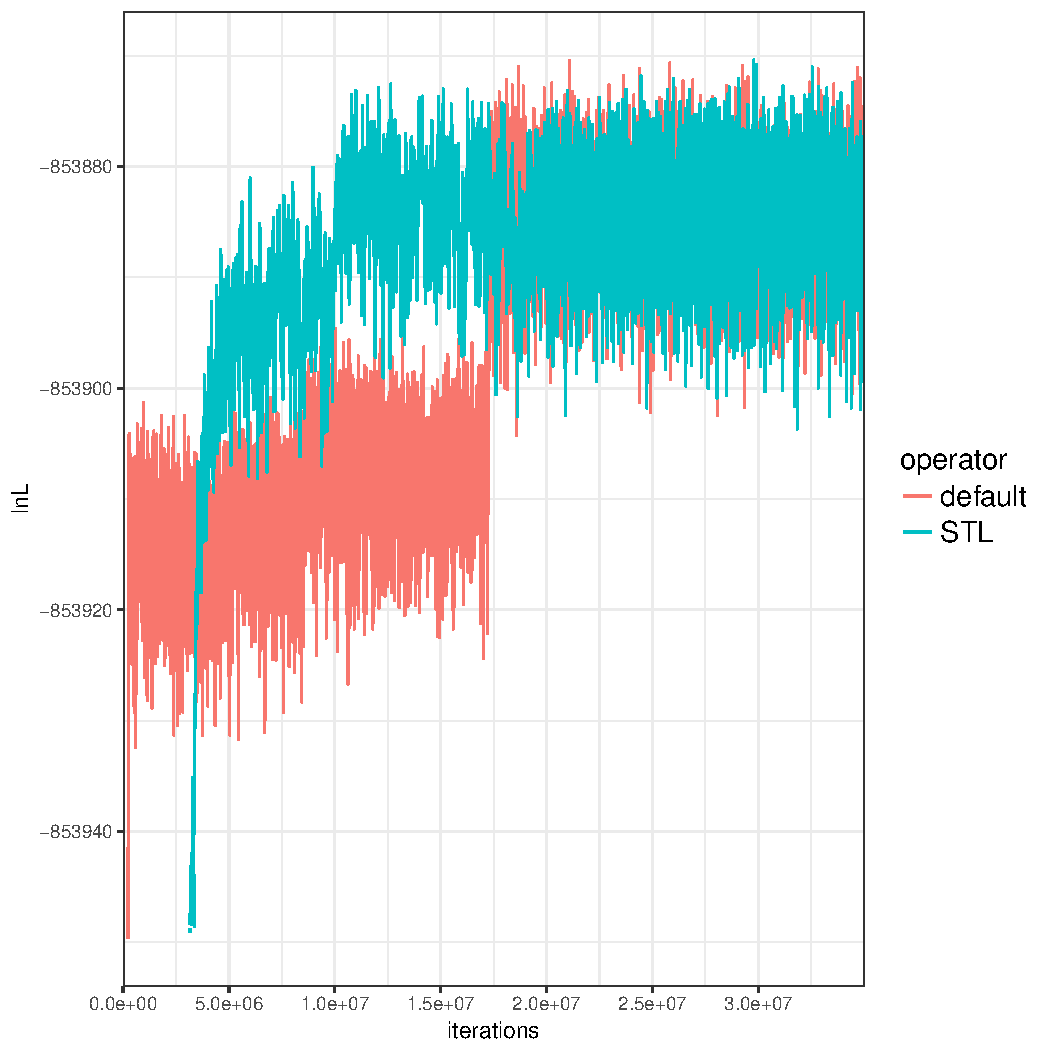
\includegraphics[width=\textwidth,height=8cm]{figures/comparison_metazoan.pdf} 
\end{figure}
\end{frame}

%-=-=-=-=-=-=-=-=-=-=-=-=-=-=-=-=-=-=-=-=-=-=-=-=
%	FRAME: end of first half
%-=-=-=-=-=-=-=-=-=-=-=-=-=-=-=-=-=-=-=-=-=-=-=-=
\begin{frame}{Hence}
SubTreeLeap seems to
\begin{itemize}
 \item explore topology space more throughly (and mix better in clade space);
 \item facilitate sampling other parameters of interest \textbf{conditional} on the tree;
\end{itemize}

Open problems:
\begin{itemize}
 \item[--] Optimal scaling: what's the optimal acceptance probability?
 \item[--] Can we construct even more efficient proposals? How to exploit structure?
\end{itemize}
\end{frame}

%-=-=-=-=-=-=-=-=-=-=-=-=-=-=-=-=-=-=-=-=-=-=-=-=
%	FRAME: Take home
%-=-=-=-=-=-=-=-=-=-=-=-=-=-=-=-=-=-=-=-=-=-=-=-=
\begin{frame}{Take home\footnote{\tiny this talk is available \href{https://github.com/maxbiostat/stats_seminar_2017}{online}}}
\begin{alertblock}{Searching trees is \textbf{hard}}
Complex, discrete and \textbf{HUGE} parameter space
\end{alertblock}\pause
\begin{exampleblock}{Height-preserving tree rearrangements are \textbf{good}}
Use the extra information provided by the tip dates
\end{exampleblock}\pause
\begin{block}{Adaptive moves are more efficient}
 Avoid wasting computing power
\end{block}\pause
\begingroup
\setbeamercolor{block title}{fg=white, bg=\cnPurple}
\setbeamercolor{block body}{bg=\cnLightPurple}
\begin{block}{Much more work is needed}
We should prepare for an era of plenty
\end{block}
\endgroup
\end{frame}

%-=-=-=-=-=-=-=-=-=-=-=-=-=-=-=-=-=-=-=-=-=-=-=-=
%	FRAME: bye
%-=-=-=-=-=-=-=-=-=-=-=-=-=-=-=-=-=-=-=-=-=-=-=-=
\begingroup
\setbeamercolor{background canvas}{bg=\cnDarkGrey}
\begin{frame}[plain]

\centering{\cGrey{\Huge{THE \newline END}}}

\end{frame}
\endgroup

\end{document}